
%\item[\hskip \labelsep {\bfseries #1}]}{\end{trivlist}}
%\newenvironment{remark}[1][Remark]{\begin{trivlist}
%\item[\hskip \labelsep {\bfseries #1}]}{\end{trivlist}}
%
%\newcommand{\fwA}{\textwidth} % one column
%\newcommand{\fwB}{0.8\textwidth} % one column
%\newcommand{\fwC}{0.5\textwidth}
%
%%%%%%%%%%%%%%%%% end of zsong's macros
%
%

\chapter{Convex Optimal Sensor Selection (COSS): An Example of Implicit Optimal Sensor Selection Method}\label{s:COSS}


%\section{Introduction}~\label{s:intro}
% Wireless sensor networks (WSNs) or smart sensor networks are key components of machine-to-machine (M2M) communication. Such networks can be used
%in a wide variety of remote monitoring and control applications that
%range from environmental and human body monitoring to military surveillance,
%building automation, industrial monitoring and control, homeland security,
%air pollution detection~\cite{LiuDualSpaceAppTracking}, wild fire
%monitoring~\cite{DoolinaFirebugSPIE05}, detection of persons and
%vehicles in open areas~\cite{DuttamirMote}, and reconnaissance
%tasks~\cite{zhao03collaborative}, etc. In typical remote monitoring applications,
%sensor nodes are scattered in an ad hoc manner over an area of interest.
%Individual sensor nodes can sense information (measurements) and communicate
%(by radio) sensed information to other sensors or to a gateway (also
%referred to as base station or sink in WSN literature). Furthermore,
%sensor nodes have a limited ability to process information on an on-board
%CPU, and can store that information in memory. This is  the reason why
%such wireless sensors are sometimes referred to as smart sensors
%or smart dust. The on-sensor processing and on-sink processing should cooperatively interpret sensor data to observe environments in energy efficient approaches. Although each individual node has limited capability, several such nodes can cooperate to accomplish complex tasks, which are called sensor fusion.
%
%    Parameter estimation is an important application for WSNs, where sensor fusion plays an important role. Many physical quantities of interest are either expensive or even impossible to measure by small sensors. For example, we may want to use several low-cost temperature sensors to estimate the position of a fire, instead of using an expensive IR camera. We may also want to use several gas sensors to locate the leaking source of certain invisible gas. The location can not be measured by a physical sensor directly.
%
%To put it succinctly, WSNs provide the ability to connect the physical world
%to enterprise computing systems, thereby improving business processes
%and facilitating efficient decision making.
%
%In many applications involving WSNs, there is a delicate trade off
%between the need to sense and communicate useful information and
%the requirement to do so in an energy efficient manner. It is expected
%that a WSN, once deployed, will work for long periods of time with
%minimal human intervention. In most remote monitoring applications,
%individual sensor nodes run on a limited supply of energy (from batteries),
%and hence, excessive on-board processing and (perhaps more importantly)
%frequent invocation of the sensors radio, rapidly depletes the sensors
%energy source. Thus, to meet these challenges, in recent years, a
%major research effort in modern computing has been devoted to the
%development of sensor network protocols and algorithms with energy-efficient
%capabilities.
%
%
%The rest of this paper is organized as follows: Section~\ref{s:prior} review the related existing solutions. Section~\ref{s:big} presents the system architecture of the proposed sensor selection method. Section~\ref{s:problemformulation} presents our formulation on the sensor selection problem.  Section~\ref{s:solution} presents our solution, the COSS algorithm. The theoretical analysis on the solution is included in Section~\ref{s:analysis}. Section~\ref{s:experiment} describes our simulations and hardware experiments.
%Section~\ref{s:diss} compares the proposed method with related methods.
%Section~\ref{s:conclusion} concludes the paper.
%% The important notation conventions are listed in the appendix. % It is recommended to read the appendix now and frequently check back while reading the paper.

\section{The Motivation and the Problem}
Parameter estimation is an important application for WSNs, where physical parameters or quantities are under estimations. Sensor fusion plays an important role for parameter estimation. Many physical quantities of interest are either expensive or even impossible to measure by small sensors. For example, we may want to use several low-cost temperature sensors to estimate the position of a fire, instead of using an expensive IR camera. We may also want to use several gas sensors to locate the leaking source of certain invisible gas. The location can not be measured by a physical sensor directly.
    Some possible applications of parameter estimation include air pollution detection~\cite{LiuDualSpaceAppTracking}, wild fire
monitoring~\cite{DoolinaFirebugSPIE05}, detection of persons and
vehicles in open areas~\cite{DuttamirMote}, and reconnaissance
tasks~\cite{zhao03collaborative}.


A fundamental problem for those applications is to balance the trade off between the need to communicate useful information and the requirement to do so in an energy efficient manner.
    It is expected that a WSN, once deployed, will work for long periods of time with
minimal human intervention. In most remote monitoring applications,
individual sensor nodes run on a limited supply of energy (from batteries), and hence, excessive on-board processing and (perhaps more importantly) frequent invocation of the sensors radio, rapidly depletes the sensors energy source.
    On the other hand, if an energy conservation policy introduces too much estimation error, then the result is not acceptable.
    Thus, to meet these challenges, in recent years, a major research effort in modern computing has been devoted to the development of sensor network protocols and algorithms with energy-efficient capabilities.


\section{Sensor Selection Problem and the Solution}\label{s:problemsolution}
\subsection{Prior Art}\label{s:prior}
 Sensor selection (or sensor scheduling) is an important technique for energy efficient observation.
    In short, the sensor selection problem is defined as selecting the ``proper'' sensors and the ``just enough'' number of sensors to observe physical phenomena. The mathematical formulations on the ``proper'' and the ``just enough'' is not unique.
    However, the concept is similar: Balance the trade off between the need for precise estimation and energy cost for communication.  For example, the ``just enough'' can be formulated as using the minimal number of sensors to send the data to the sink, subject to bounded estimation errors~\cite{SAM2006Amit}. It is also possible to formulate the ``just enough'' as minimizing communication costs by sending only the non-redundant sensor information through the communication channel. The physical phenomena are estimated based on the less redundant data~\cite{FZhaoShinInfoDrivenDynamicTracking}. In this chapter, we argue that the minimum number of sensors that allowed by the Carath\'{e}odory's theorem is ``just enough'' to approximate the most precise estimate: The Cram\'{e}r-Rao lower bound (CRLB).


Note that the brute force sensor selection approach is too expensive, in term of computation and hardware costs. Each sensor has two states: selected and unselected. Thus, the solution space for $n$ sensors has $2^n$ states. This is a NP hard problem~\cite{isler06tase} and it is impossible to use the brute force approach in practice.

The sensor selection problem has been discussed from different aspects in the literature. Our classification on the existing sensor selection methods is shown in Fig.~\ref{f:ssChart}. Our proposed COSS method is an implicit optimization method. Hereby we briefly describe each method and compare them with our proposed method. For presentation purposes, we use a lamp tracking scenario has the example, even though our method is applicable to more general parameter estimation problems. In our scenario, sensor nodes equipped with light sensors are placed on a table. A lamp is placed at a constant height above those sensors and can be moved by hands. The task is to track the position of the lamp based on the data collected by those light sensors. We assume that the locations of the sensors are known.~\footnote{Although the sensor positions are required by the sensor selection algorithms, the sensor localization problem and the sensor selection problem are mostly independent. It is common for sensor selection papers to assume that the positions of the sensors are known~\cite{isler06tase,SAM2006Amit,FZhaoShinInfoDrivenDynamicTracking,UcinskiPatanDoptSensorSelection06}.}


On the highest level of Fig.~\ref{f:ssChart}, there are semantic and numerical methods. From the database aspect, the semantic method considers the sensor selection as a semantic routing problem~\cite{GehrkeQueryProc2004,madden02design}. This method can select sensors based on properties of the sensor nodes, or simple properties of the sensor data. For example, the method is capable to select ``all sensors on the 4th floor'' or ``all sensors who detect high temperature''~\cite{GehrkeQueryProc2004}. This problem is essentially formulated as a tree search problem~\cite{madden02design}. Our application scenario is different: There is no simple threshold to choose the proper sensors. For example, if several sensors are close to each other and have high light values, we may choose just one out of them since much of their sensor data are redundant. There is no simple threshold method to tell which sensor data is better.


Numerical methods select the proper sensor based on quantitative computations. Sensors can be selected based on the intrinsic properties of their measurements, or the other sensors' measurements, based on sensor fusion technologies.
    The model free methods do not require models of the physical world. For example, utility-based sensor selection methods~\cite{byersUtilSS,utility-based-sensor-selection} select sensors by maximizing utility functions. Our method is model based, thus different.


There are also many model-based sensor selection methods, by which the physical models are used. Since many physical quantities are distributed and subject to physical laws, some sensor data can be inferred from other data. Given the model, it is not necessary to estimate physical phenomena with all the sensor data.


A model based geometric method is presented in paper~\cite{isler06tase}.
Based on geometrical analysis on camera-like sensors, the paper concludes that the sensor selection problem can be solved in polynomial time. The paper also observed that ``the estimates that obtained by four sensors are as good as the estimates obtained form all sensors.'' This observation is in consistent with the algebraic analysis in this chapter. Section~\ref{s:analysis} presents more details.


Sensor selection problem can be studied from the aspect of information compression: The sensor data with high uncertainty or redundancy should not be transmitted via the communication channel. The uncertainty is measured by entropy and the redundancy can be measured by correlations. For example, the paper~\cite{FZhaoShinInfoDrivenDynamicTracking} presents a sensor selection method based on the entropy filtering and Bayesian theorem. This is a grid-based method: The area of interest is segmented into many small cells, and the entropy of the target's location is computed based on the probability mass function. Since smaller entropy indicates less uncertainties of the information, paper~\cite{FZhaoShinInfoDrivenDynamicTracking} proposes an algorithm to select proper sensors by minimizing the entropy. Thus, only the ``good'' information with more certainties is sent to the sink. The probability mass function can be recursively updated according to the dynamics of the target. The updating method is based on the Bayesian theorem. More details of this method is presented in~\cite{liu02collaborative,zhao03collaborative,ZhaoGuibasWSN2004}. Based on the same framework, paper~\cite{wang04entropybased} proposes a faster heuristic entropy-based sensor selection method.


Comparing to the above methods, our proposed sensor selection is significantly different. 1) Our proposed method is not grid-based. 2) Our method minimizes estimation error, instead of uncertainties in sensor data. 3) Our method implicitly minimizes the number of selected sensors and explicitly minimizes the estimation error.


    Another example of the information compression approach is present in~\cite{VuranSpatioTemporal04}, where sensors are directly deployed to measure the physical quantity of interest. The measurements are subject to a tempo-spatial correlation model. The variance of the estimation noise is minimized by selecting proper sensors.
    Our application scenario is different: Firstly, we are interested in parameter estimation problem, where the quantity of interest can not be directly measured by sensors. Secondly, we observed from experimental data that our sensor data should be considered uncorrelated. Figure~\ref{f:sensorIID} is a plot of a $11\times 11$ correlation coefficients matrix for the light sensors on Tmote Sky~\cite{TmoteSkyDS2006} sensor nodes. In the experiment, we uniformly placed 11 sensors under a lamp at different distances. Figure~\ref{f:sensorIID} shows that the magnitudes of the cross-correlations between two sensors at different distances are much smaller than that of the auto-correlations (the diagonal values in the figure). In fact, the mean of the cross-correlation coefficients of the experiment data is only $0.1181$. Thus, our sensor data should not be considered correlated.
    Our sensor selection method does not depend on cross-correlations and we have verified our sensor selection method on our hardware testbed, which is based on Tmote Sky sensor nodes.


\begin{figure}
  % Requires \usepackage{graphicx}
  \centering
  \includegraphics[width=\fwB]{img/SSChart}\\
  \caption{A classification on sensor selection methods.}\label{f:ssChart}
\end{figure}


\begin{figure}
  % Requires \usepackage{graphicx}
  \centering
  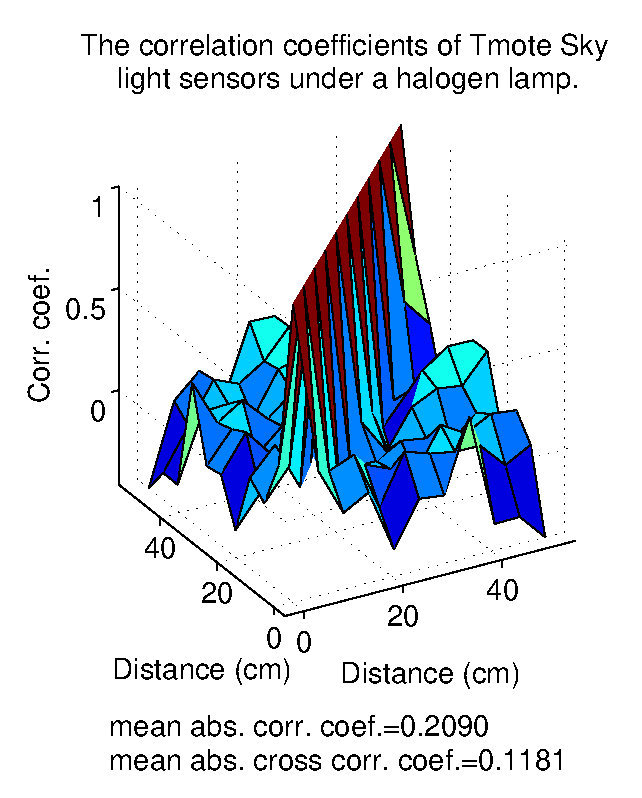
\includegraphics[width=\fwC]{img/HalogenCorrCoef}\\
%  \includegraphics[width=3.5cm]{img/ExpCorrCoef}\\
  \caption{The correlation coefficients of Tmote Sky light sensors. (Based on our hardware experiment data.)}\label{f:sensorIID}
\end{figure}


Sensor selection can be discussed within the framework of optimal estimation, where the estimation error is normally used as the cost function of the optimization. In previous works~\cite{SAM2006Amit,Fusion2005Amit,JafariGASensorSelectionInformationSciences2001} and~\cite{UcinskiPatanDoptSensorSelection06}, the sensor selection problem is formulated as a constraint 0-1 integer programming problem, where the estimation error is minimized. The number of sensor is given and used as the constraints. In~\cite{SAM2006Amit}, the sensor selection is formulated as a 0-1 integer programming (or binary integer programming) problem and solved by a branch and bound (B\&B) method. In~\cite{JafariGASensorSelectionInformationSciences2001}, the sensor selection problem is formulated as a combinatorial optimization problem as well as a binary integer programming problem. The problem is solved by a GA (genetic algorithm) software.
 Those methods are closest to our proposed method, but the difference is still obvious: Our method does not explicitly minimize or choose the number of selected sensors.


Our method is an example of the implicit optimization. The feature of this class of methods is that the number of selected sensors is not explicitly shown in the cost function or constraints of the optimization. Instead, the number of selected sensors is minimized simultaneously during the time when estimation error is minimized. It is desirable and may be counter-intuitive. Using the minimum number of sensors, the least estimation error can be achieved! Selecting more sensors does not necessarily improve the estimation precision. Rather, more properly scheduled sensors can cover a larger area for observation. Before presenting the details in Section~\ref{s:problemsolution}, we summarize the key features of our method: (1) Simultaneously achieve the optimal estimate with the least number of sensors, as well as the least energy costs. No compromise is required between the estimation precision and energy cost. (2) Simple and fast. (3) The robustness of the method has been verified by extensive hardware experiments.


\subsection{Overview on Our Strategy}\label{s:big}
    As aforementioned, the sensor selection problem is NP hard. Thus, our strategy is to simplify the problem by several reasonable approximations and solve the approximated problem by a fast optimization approach.


     We do not add the two cost functions (cost for estimation errors and number of selected sensors) together and minimize the summation, or construct a vector based on the cost functions. These are standard multi-objective or combinatorial optimization techniques. Instead, we only minimize the cost function that associated with the estimation error. However, the number of selected sensor is automatically minimized during the time when we minimize the estimation error. This is due to the fact that we intentionally select a proper convex cost function and it has a convex constraint. According to the Carath\'{e}odory's theorem, the number of selected sensors is minimized. The details are presented in the Section~\ref{s:analysis}.


% In short, we want to kill two birds with one stone. That is, we want to approach both the lowest estimation error bound, which is limited by Cram\'{e}r-Rao lower bound (CRLB) in theory, and the minimum number of selected sensors that allowed by the Carath\'{e}odory's theorem.


  We do not add the two cost functions (cost for estimation errors and number of selected sensors) together and minimize the summation, due to the high computation cost of integer programming. Remind that the number of selected sensors is an integer.  Thanks to the gradient, the computation costs of continuous optimization problems are normally much less than the of the integer programming problems.
  %   Normally, the computation cost to minimize an integer cost function is much higher than that of continuous cost function.
  % It will take much more computations to minimize that cost function than our proposed, continuous cost function.


The system block diagram of our proposed method is shown in Fig.~\ref{fig:sysmodel}, where the physical parameter $\mathbf{q}^\ast$ is the position of lamp, $y_{i}$ is the nominal light value, $v_{i}$ is the sensor measurement noise, and $s_{i}$ is the sensor reading.
    Note that our convex optimal sensor selection (COSS) algorithm includes the three blocks on the right, i.e., ``wireless sensor network,'' ``least squares fitting,'' and ``optimal sensor selection.'' As we can see in Fig.~\ref{fig:sysmodel} that the three blocks interact on each other, and they are inter-dependent. Thus, all the blocks are included in our COSS algorithm, which is list in Algorithm~\ref{a:COSS}, Section~\ref{s:solution}. The ``wireless sensor network'' is associated to part 1 of the Algorithm~\ref{a:COSS} and carried out on individual sensor node. The part 2 in the Algorithm~\ref{a:COSS} is referring to the other two blocks, i.e., ``least squares fitting,'' and ``optimal sensor selection,'' in Fig.~\ref{fig:sysmodel}. The part 2 is the task for the sink.

\begin{figure*}
\begin{center}\includegraphics[%
%  width=\linewidth,
  width=\fwA,
  keepaspectratio]{img/CentEDSysBlock}\end{center}
\caption{System block diagram of the proposed method.\label{fig:sysmodel}}
\end{figure*}


% In this system architecture, the WSN is not a passive sensing device. The sampling rate of the WSN is adapted according to the estimate $\mathbf{\hat{q}}$. The sensors and the sink interactively adjust the sampling rate for optimal estimation.
% After actively adjust its sampling rate, the data collected by the WSN is changed, which future affect the estimate $\mathbf{\hat{q}}$. Thus, if the system continuously updates the sample rate value, it is essentially a closed-loop control problem, and the stability must be guaranteed. In this


The future working scenario is shown in Fig.~\ref{f:scenario}.
In the figure, a target tracking scenario is demonstrated. However, the
method is applicable to generic parameter estimation problems.
After a target appears on the field of view, a subset of
the sensor nodes observe the event and start measuring the
physical quantity (light, temperature, gas concentration etc)
that is associated with the target. At the beginning, many
the sensor nodes detect the target and they enter an active mode.
Their sampling rates and transmission rates are levitated to a high level, as shown in Fig.~\ref{f:scenario}(A).
Although the transmission rate is high, not too much energy is
required, since this initial stage does not last for a long time.
    Soon, several sensors are selected to stay in the active mode
    and continuously monitor the target.
    Other sensors switch back to the inactive mode. Their sampling rates and transmission rates are considerably lower.
    One elected leader sensor among the
    active sensors takes the responsibility to report monitoring data to the sink.
    All these operations should be distributed, in future. This case is shown in
    Fig.~\ref{f:scenario}(B).
        As the target moves, the selected sensors smoothly shift from one to another. This
        is shown in Fig.~\ref{f:scenario}(C).
            Our current hardware implementation is presented in Section.~\ref{s:experiment}. Although the current implementation is not at the level of this future working scenario, the experiment indicates that the proposed COSS algorithm is fast and memory efficient. It has potentials to be implemented on low cost sensor nodes.
%Once data starts arriving at the sink, the
%rough position of the target can be estimated through a least squares
%optimization program running on the sink. Based on
%this rough position estimate, only some subset of sensor nodes are selected
%and continue to be assigned high sampling rates, while others are unselected
%and virtually stop sampling and packet transmission in order to conserve precious
%on-board battery energy. The process continuously refines
%the position estimate and then selecting different sensors based on the
%track of the target. This is shown in Fig.~\ref{f:scenario}(b).
%Note that, the same scheme can be adopted to estimate other
%target parameters. For example, in addition to the location of
%an illumination source, it might be required to estimate the
%strength of the illumination source as well. In future work,
%alongside the problem of sampling rate assignment, we plan
%to consider efficient routing of packets from sensor nodes to
%sink as shown in Fig.~\ref{f:scenario}(c).


\begin{figure*}
%\begin{center}\subfigure[A target appears.]{\includegraphics[%
%  width=0.3\linewidth,
%  keepaspectratio]{EventObs1.eps}}\subfigure[Select sensors.]{\includegraphics[%
%  width=0.3\linewidth,
%  keepaspectratio]{EventObs2.eps}}\subfigure[Sensor data are route to the sink.]{\includegraphics[%
%  width=0.3\linewidth,
%  keepaspectratio]{EventObs3.eps}}\end{center}
\centering
\includegraphics[width=\fwA]{img/COSSScenario}
\caption{The WSN sensor selection working scenario.\label{f:scenario}}
\end{figure*}

    As aforementioned, the original sensor selection problem has a large solution space and it is hard to solve. Thus, our strategy is to simplify the problem by several reasonable approximations and solve the approximated problem by a fast optimization approach.
% In short, we want to kill two birds with one stone. That is, we want to approach both the lowest estimation error bound, which is limited by Cram\'{e}r-Rao lower bound (CRLB) in theory, and the minimum number of selected sensors that allowed by the Carath\'{e}odory's theorem.


%\subsection{Background Knowledge:Fisher information}~\label{s:fi}
%%% moved to the appendix
%Fisher information is a metric to indicate the sensitivity of the measurements with respect to system parameters.
%%\begin{mdef}\label{d:fisher}
%%If a measurable random variable $X$ depends on parameter $\theta$, and the likelihood function is $l(\theta;X)$.
%%Then the Fisher information is
%%\begin{equation*}
%%    \mathcal{I}=E\{[\frac{\partial}{\partial \theta} \log l(\theta;X)]^2 \}
%%\end{equation*}
%%The matrix form is Fisher information matrix, which is $M$, with the $i,j$th entry defined as:
%%\begin{equation*}
%%    M_{(i,j)}=E\{\frac{\partial}{\partial \theta_i} \log l(\theta;X) \frac{\partial}{\partial \theta_j} \log l(\theta;X) \}
%%\end{equation*}
%%\end{mdef}
%
%Easy to see, if $P_r(X;\theta)$ is independent Gaussian, the sensitivity for each sensor can be computed separately.
%% Eq.~\ref{e:m} is the Fisher information matrix.
%\begin{eqnarray*}
%% \nonumber to remove numbering (before each equation)
%  l(\theta;X) &=& \frac{1}{\sqrt{2\pi}\sigma} \exp(-\frac{(X(\theta)-\mu)^2}{2\sigma^2})\\
%  M_{(i,j)} &=& E\{\frac{\partial}{\partial \theta_i} \log l(\theta;X) \frac{\partial}{\partial \theta_j} \log l(\theta;X) \} \\
%%  M_{(i,j)}&=& E\{\frac{\partial}{\partial \theta_i}(-\ln(\sqrt{2\pi\sigma^2})-\frac{(X(\theta)-\mu)^2}{2\sigma^2})
%%    \frac{\partial}{\partial \theta_j}(-\ln(\sqrt{2\pi\sigma^2})-\frac{(X(\theta)-\mu)^2}{2\sigma^2}) \}\\
%  M_{(i,j)} &=& E\{\frac{(X-\mu)^2}{\sigma^4}\frac{\partial X}{\partial \theta_i}\frac{\partial X}{\partial \theta_j} \} \\
%  M_{(i,j)} &=& \frac{1}{\sigma^2} \frac{\partial X}{\partial \theta_i}\frac{\partial X}{\partial \theta_j}
%\end{eqnarray*}
%Thus, (\ref{e:m}) is the Fisher information matrix.
%
%%A related concept is Fisher information entropy. Paper~\cite{RomeraFisherEntropy99} formulates Fisher information entropy for a 3D particle system as $\mathcal{I}_f$,
%%\begin{equation}\label{e:fentropy}
%% \mathcal{I}_f = \int [\|\nabla f(\mathbf{r})\|^2 /f(\mathbf{r}) ] \hbox{d}\mathbf{r},
%%\end{equation}
%%where $f(\mathbf{r})=f(x,y,z)$ is the pdf for a particle appears at the position $\mathbf{r}$.
%
%
%\begin{thm}[Cram\'{e}r-Rao inequality \cite{MoonSig} pp.551]
%If $t(\theta)$ is any unbiased estimator of $\theta$ based on a differentiable likelihood function, then
%\begin{equation} \label{e:crlb}
%    E\{(t(\theta)-\theta) (t(\theta)-\theta)^T\} \geq M^{-1}(\theta),
%\end{equation}
%where $M(\theta)$ is the Fisher information matrix (FIM).
%\end{thm}
%\begin{remark}
%According to this theorem, the inverse of the FIM is the indicator for the minimum possible covariance of any unbiased estimators. In fact, if the maximum likelihood estimator, $\theta_{ML}$, exists, the following equation holds~\cite{EmeryOED98}:
%$$E\{(\theta_{ML}-\theta)(\theta_{ML}-\theta)^T\}=M^{-1}(\theta). $$
%In other words, reducing the right hand side of (\ref{e:crlb}) actually improves the estimator $\theta_{ML}$, if it exists.
%%if we can find an unbiased estimator $\bar{t}(\theta)$ achieve the CRLB, or $ E\{(\bar{t}(\theta)-\theta) (\bar{t}(\theta)-\theta)^T\} = M^{-1}(\theta)$, then $\bar{t}(\theta)$ is called efficient.
%%    Although it is possible that a biased estimator has less error
%%If we have a
%\end{remark}



\subsection{Problem Formulation}\label{s:problemformulation}
% Our method follows the framework of experiment design and it is applicable to general parameter estimation problems, not just limited to the target tracking. However, for presentation purpose, we use a lamp tracking case has the example to interpret our formulation. This is the exact working scenario of our hardware testbed.

    Assuming the true position of the lamp at the time instance $k$ is $\mathbf{q^\ast}[k]$, and the position of the $i$th sensor is $\mathbf{r}_i$. The following equations hold:
\begin{eqnarray*}
    y_i[k] &=& f(\mathbf{q^\ast}[k]; \mathbf{r}_i), i=1,2,\cdots,n ;\label{e:yfq} \\
    s_i[k] &=& y_i[k]+v_i[k].\label{e:syv}
\end{eqnarray*}
where $f$ is the sensor model, $y_i[k]$ is the nominal reading from the $i$th sensor, and the associated real sensor reading is $s_i[k]$, which is corrupted by the independent Gaussian noise $v_i[k]$. In this chapter, we use a common energy model~\cite{ArandaOptSensorPlacement05} as the sensor model.


\begin{mdef}[Energy Model]
\begin{eqnarray}
% \nonumber to remove numbering (before each equation)
  y_i[k] &=& \frac{c_1}{h^2+d_i^2[k]}, \label{e:ynormal} \\
  v_{i}[k] & \thicksim & \mathcal{N}(0,\sigma),\nonumber \\
  d_i[k] &=& \| \mathbf{r}_i-\mathbf{q^\ast}[k] \| , \nonumber
\end{eqnarray}
  where $h$ is the height of the lamp, $d_i[k]$ is the distance from the sensor to the exact position under the lamp, $c_1$ is a constant, and $\sigma$ is the standard deviation.
\end{mdef}

\begin{remark}
The energy model can be reasonably interpreted by physics. The fact that the sensor can observe the target indicates there is energy come from the target being detected by the sensor. The energy emitted from the target is uniformly spread in space and propagates in spheres. Thus, the energy density is proportional to $1/r^2$, where $r$ is the radius of the sphere, or the distance from the target to the sensor. Under ideal conditions, if the sensor characteristics are linear, i.e., the sensor reading is proportional to the energy it received, then the energy model holds.

% The energy model is constructed based on physical properties. Fig.~\ref{f:EnergyModel}(a) illustrates why the nominal measurement is proportional to inverse of the distance square. The light bulb in Fig.~\ref{f:EnergyModel}(a) indicates a target which broadcast energy to the free space. A reasonable assumption is that the sensor's nominal measurement is proportional to the energy density. If the energy is emitted at a constant rate, then the summations of the energy on spheres of different radii are equal. Since the surface area of the sphere is $4\pi r^2$, the sensor's nominal measurement is $c_1/r^2$.


The configuration scenario of the energy model is shown in Fig.~\ref{f:EnergyModel}, where the target is on top of the plane that the sensor lay on. Easy to see that $r^2$ can be replaced by $h^2+d^2$. Thus, (\ref{e:ynormal}) is derived.

\begin{figure}
  \centering
%  \subfigure[Free space energy model.]{\includegraphics[width=4cm]{img/EnergySurf}}
%  \subfigure[Generic settings of energy model.]{\includegraphics[width=7cm]{img/LampEnergyModel}}
%  \caption{Configuration of energy model.}\label{f:EnergyModel}
  \includegraphics[width=7cm]{img/LampEnergyModel}
  \caption{Generic settings of energy model.}\label{f:EnergyModel}
\end{figure}


In the simulations of this chapter, we use the following constants
\begin{itemize}
  \item $c_1=3.3032\times 10^6$,
  \item $h=20.32$ cm.
\end{itemize}
\end{remark}
These parameters are chosen such that the energy model approximates the data measured by experiments.

\begin{mdef}[Polynomial Model]~\label{d:poly}
\begin{eqnarray*}
   y_i[k] &=& \left\{
  \begin{array}{ll}
    c_2 + c_3 d_i[k] + c_4 d_i^2[k], & \hbox{$y_i[k]\geq y_L$,} \\
    Invalid, & \hbox{otherwise,}
  \end{array}
\right.\\
  v_{i}[k] & \thicksim & \mathcal{N}(0,\sigma_i[k]),\\ %\label{eq:ynormal} \\
  \sigma_i[k] &=& \left\{
                    \begin{array}{ll}
                      c_5+c_6 d_i[k] + c_7 d_i^2[k], & \hbox{$y_i[k]\geq y_L$,} \\
                      Invalid, & \hbox{otherwise,}
                    \end{array}
                  \right. \\
  d_i[k] &=& \| \mathbf{r}_i-\mathbf{q^\ast}[k] \| ,
\end{eqnarray*}
where $c_2$ to $c_7$ are constants, and $d_i[k]$ is the distance from the sensor to the exact position under the lamp.
\end{mdef}
\begin{remark}
The polynomial model is characterized based on our hardware experiment data. The data are plot in Fig.~\ref{f:SensorFit}. The left plot in the figure is the light value with respect to the distance, measured by cm. While the right plot is the standard deviation with respect to the distance. Note that the value of the standard deviation depends on the distance, in practice. In the figure, it is seen that the fitting errors of the polynomial model are relatively small.

The experiment data can be fitted by the energy model. However, the fitting error is larger than that of the polynomial model. This may due to the nonlinear characterizes of the sensors.

In the hardware implementations, we use the following parameters:
\begin{itemize}
  \item \begin{tabular}{ccc}
          % after \\: \hline or \cline{col1-col2} \cline{col3-col4} ...
          $c_2=6720.0,$ & $c_3=-216.0,$ & $c_4=2.524,$ \\
        \end{tabular}
  \item $\; y_L=2500$,
  \item \begin{tabular}{ccc}
          % after \\: \hline or \cline{col1-col2} \cline{col3-col4} ...
          $c_5=824.0,$ & $c_6=-36.26,$ & $c_7=0.4577.$ \\
        \end{tabular}
\end{itemize}

In the model, ``invalid'' means that the optimization for sensor selection does not consider the invalid sensors. Just as if those invalid sensors are not exist. The $y_L$ is the threshold where the ambient light is more significant than the lamp's light. In Fig.~\ref{f:SensorFit}, $y_L$ is about 35 cm.
\end{remark}

\begin{figure}
  \centering
%  \subfigure{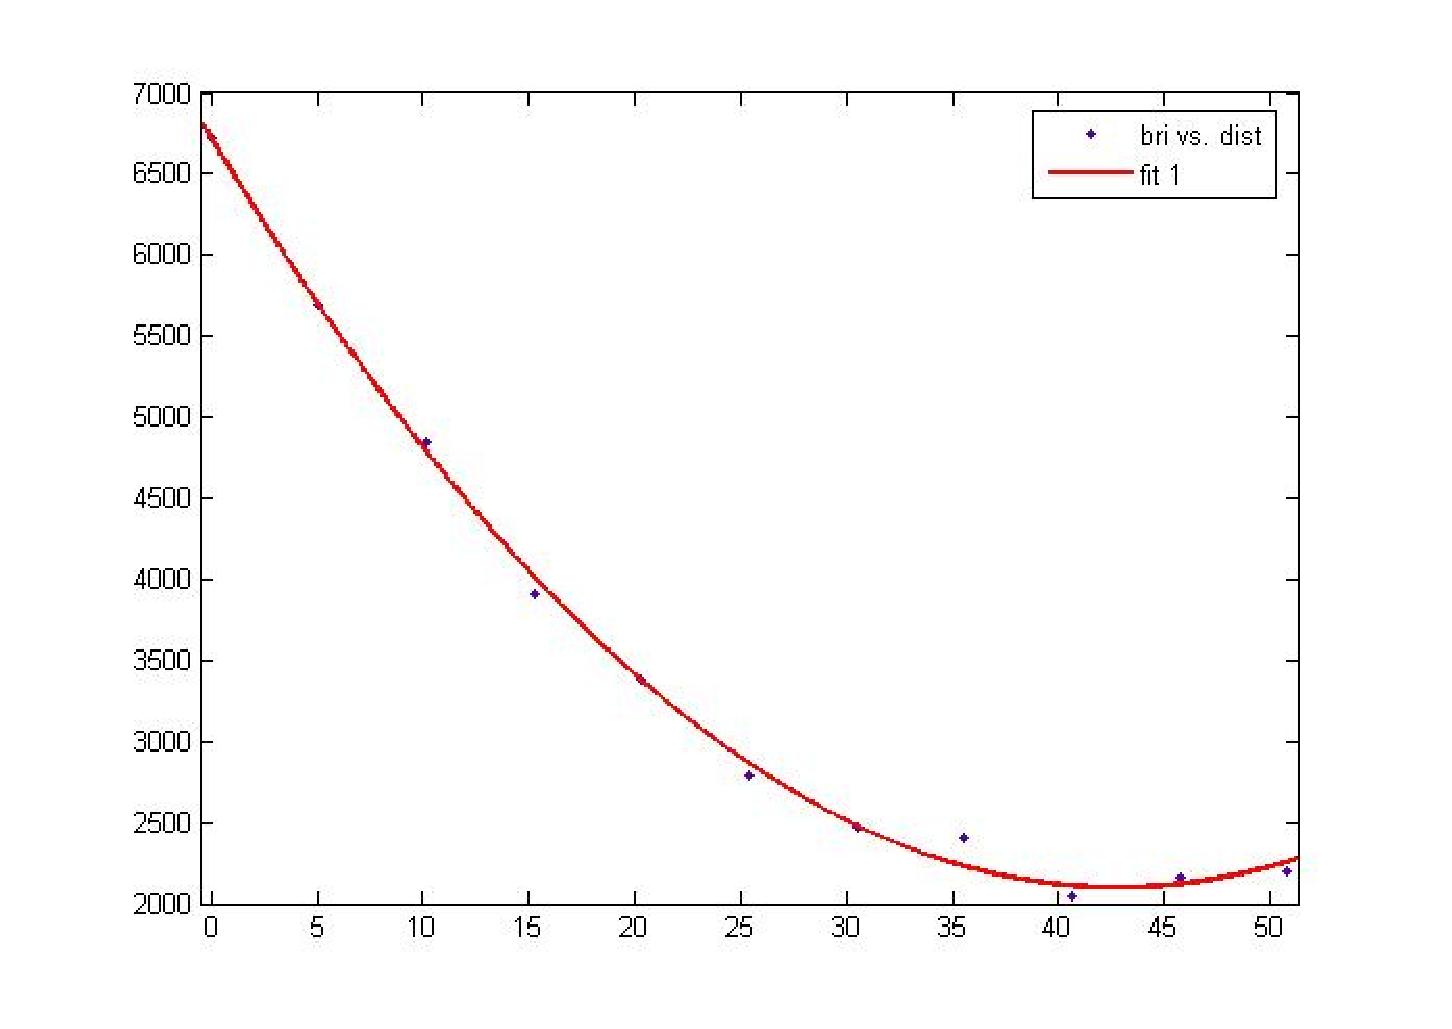
\includegraphics[width=6cm, height=6cm]{img/SensorFit2DOct02Quad}} %
%  \subfigure{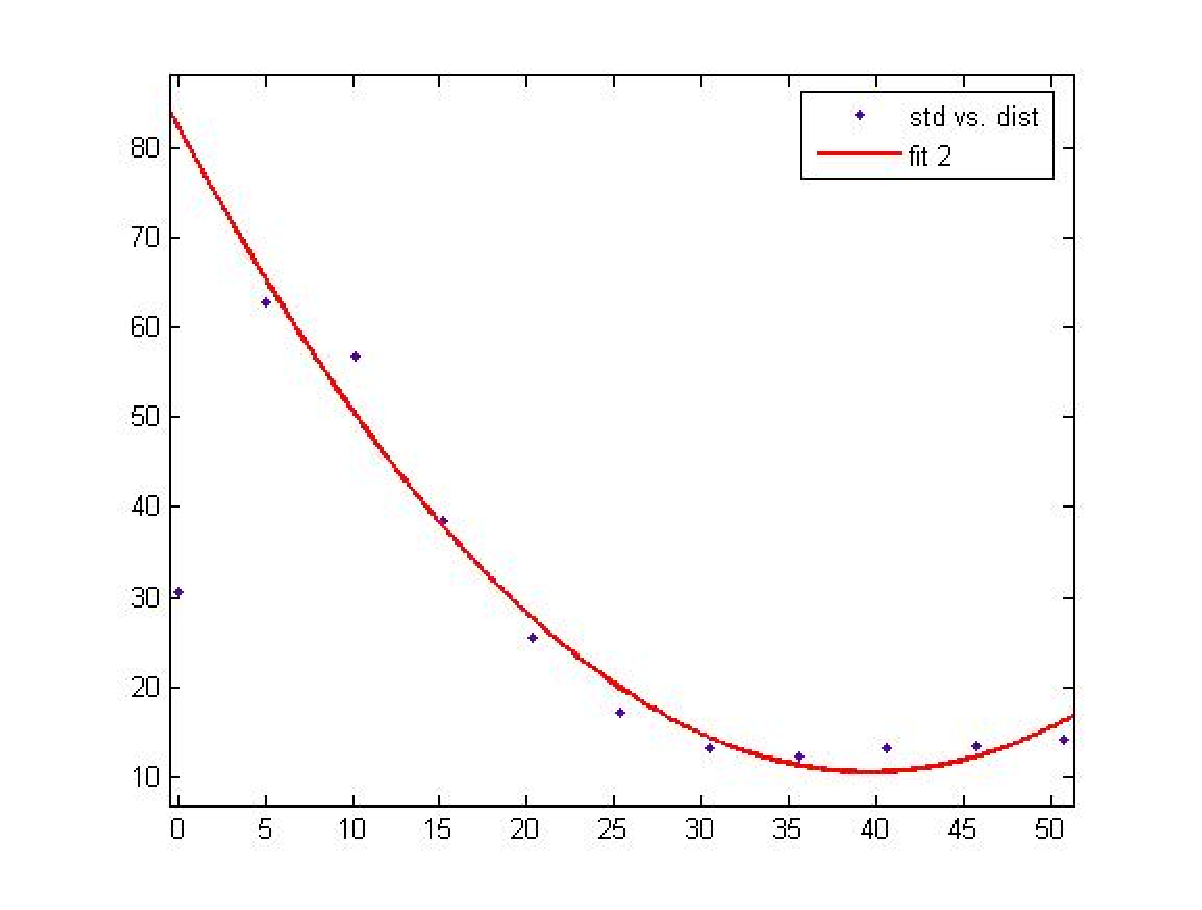
\includegraphics[width=6cm, height=6cm]{img/SensorFit2DOct02StdQuadRobust}}
  \subfigure{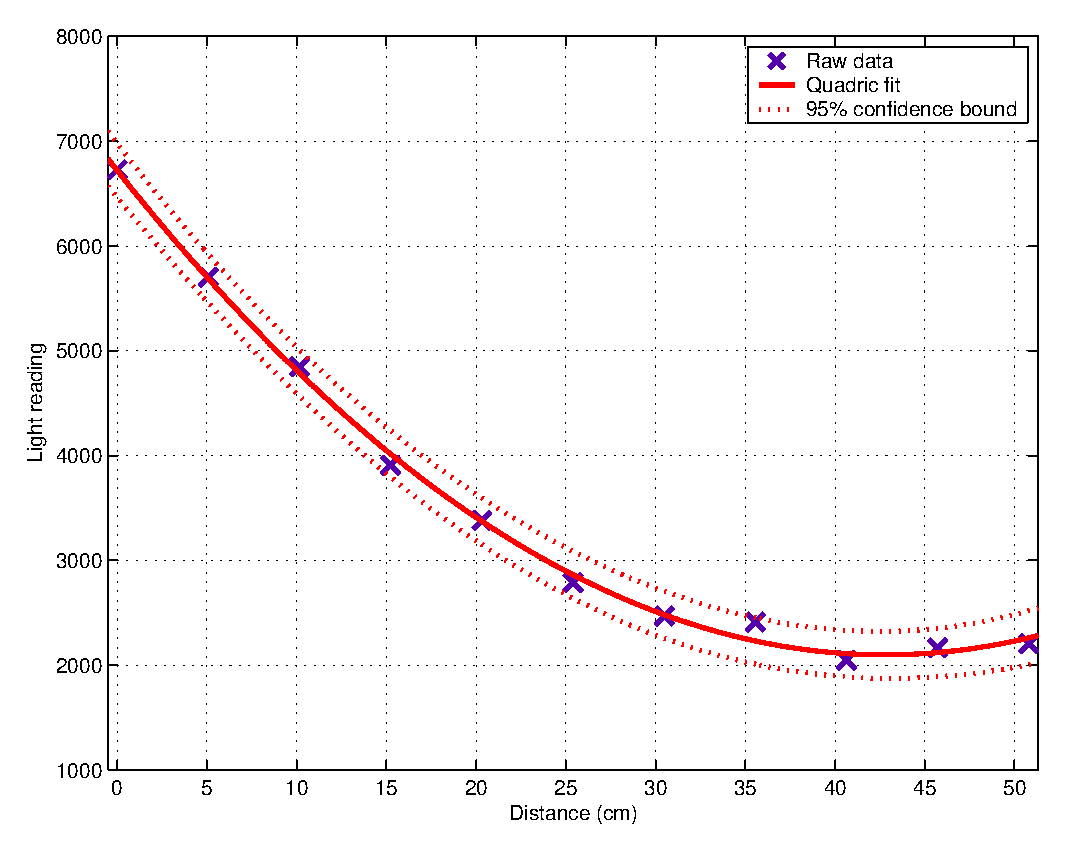
\includegraphics[width=6cm, height=6cm]{img/RangeLightFit}}
  \subfigure{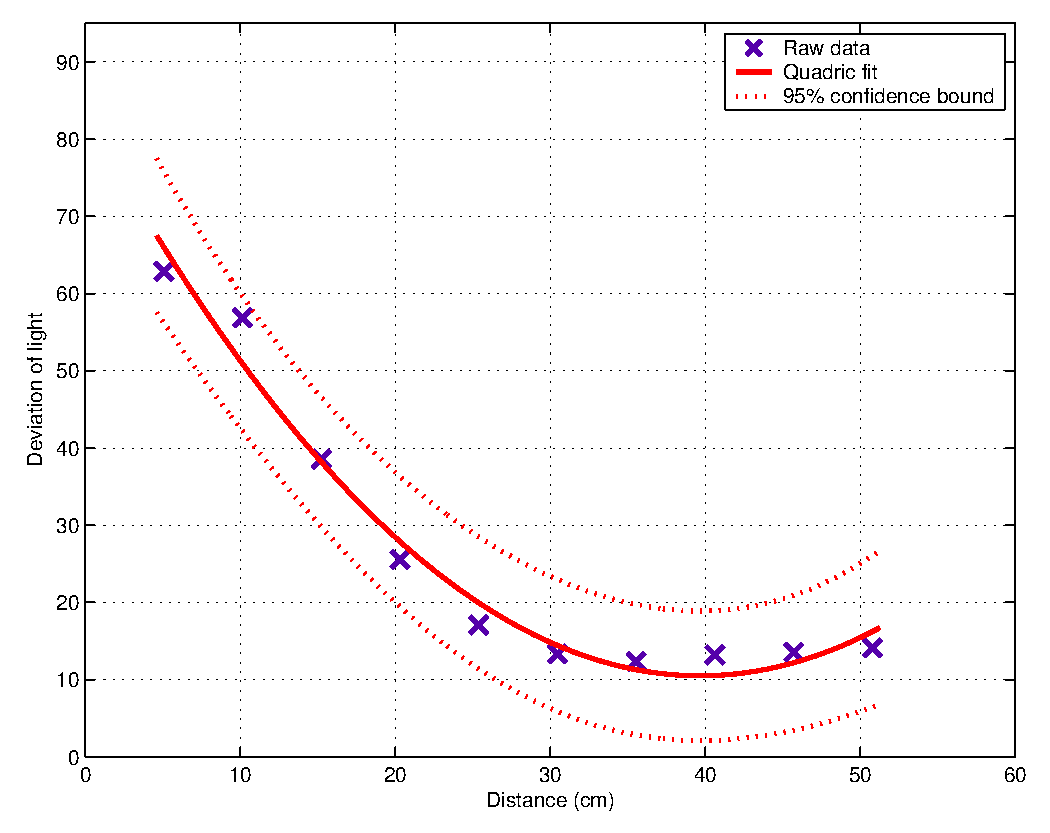
\includegraphics[width=6cm, height=6cm]{img/RangeStdFit}}
  \caption{The characteristics of the light sensors on Tmote Sky.}\label{f:SensorFit}
\end{figure}


In order to reduce the noise $v_i$, the $i$th sensor node measures the $n_i$ light values in the time slot $t_S$, averages them and sends the averaged value back to the sink. The averaged light value is $\bar{s}_i[k]$, whose standard deviation is smaller than that of the raw data:
$$\bar{\sigma}_i^2[k]=\sigma_i^2[k]/n_i.$$
 If we can afford infinite number of samples, we can reject the noise totally. Of course, there is an upper limit on sample number in practice. For simplicity, we set $n_S$ as the upper limit on the total number of samples for all the sensors in the time slot $t_S$.
    The intuitive interpretation is as follows.
We estimate the position of an event based on sensor measurements.
Since sensor measurements are noisy, the event observations are not perfect.
Now, noise in the sensor measurements can be reduced by modifying the sensor design (use better hardware) or by filtering
away sensor noises. Given fixed hardware, a simple filtering technique to adopt is to average the sensor data.
%In the latter approach, one possible option is to take a large number of sensor measurements (samples) and then average them by each sensor to eliminate as much noise as possible.

After receiving all the sensor data, the sink estimates the lamp's position by the standard nonlinear least squares (LS) method, and the output is $\hat{\mathbf{q}}_A$, which is also called the a priori position. For a network of $n$ sensors, the $\hat{\mathbf{q}}_A$ is as (\ref{e:qA}).
\begin{equation}\label{e:qA}
    \hat{\mathbf{q}}_A[k] = \mathrm{argmin}_{\mathbf{q}} \frac{1}{2} \sum_{i=1}^{n} (\bar{s}_i[k]-y_i(\mathbf{q}; \mathbf{r}_i))^2.
\end{equation}



Now, we introduce several approximations to simplify the problem.
\begin{itemize}
  \item Instead of assigning each sensor a binary value that indicates the ``selected'' or ``unselected'' state, we assign a normalized sampling rate $p_i$ to sensor $i$. That is, $$p_i[k]\in [0,1] \;\mathrm{ and } \sum_i p_i=1.$$ Thus, the integer programming problem is approximated by a continuous design problem.
       \item Our cost function is based on the Fisher information matrix (FIM), $M$, whose inverse matrix is the Cram\'{e}r-Rao lower bound (CRLB)~\cite{CheungLSTOA04,UcinskiOptDPS05}.
   The definition of Fisher information and FIM is presented in Appendix.~\ref{s:fi}.
    Ideally, the optimal sampling rate is
    $$\mathbf{p}^\ast[k]=\mathrm{argmin}_{\mathbf{p}} \Psi(M(\mathbf{p};\mathbf{q}^\ast[k])).$$ Since $\mathbf{q}^\ast[k]$ is unknown, we replace it by $\hat{\mathbf{q}}_A[k]$, which is another approximation. Thus, $$\hat{\mathbf{p}}[k]=\mathrm{argmin}_{\mathbf{p}} \Psi(M(\mathbf{p};\hat{\mathbf{q}}_A[k])).$$
        \item The nonlinear sensor models are linearized as $\mathbf{y}[k] = A^T \hat{\mathbf{q}}_A[k].$ This is a common approximation technique.
\end{itemize}
Thus, we simplified the original problem to the following sampling rate optimization problem.
\begin{mdef}[Sampling Rate Optimization Problem]\label{d:SampRateOpt}
\begin{eqnarray}
 \hat{\mathbf{p}}[k]  &=&  \mathrm{argmin}_{\mathbf{p}} \Psi(M(\mathbf{p}; \mathbf{\hat{q}}_A[k])),  \label{e:pk}\\
% \Psi(M) &=& -\ln\det(M), \label{e:dopt}\\
 \hbox{\rm subject to} :  \mathbf{p} &\geq& 0 ,  \nonumber \\
 \mathbf{1}^{T}\mathbf{p} & = & 1 , \nonumber \\
 \mathbf{y}[k] &=& A^T \hat{\mathbf{q}}_A[k],\nonumber \\
 A &=&  \nabla_{\mathbf{q}}\mathbf{y}|_{\mathbf{q}=\mathbf{\hat{q}}_A[k]}, \label{e:defA} \\
 M &=&  A \Sigma^{-1}A^T , \label{e:mSSP}\\
 \Sigma^{-1} & =& \left[\begin{array}{ccc}
        \tilde{\sigma_{1}}^{-2}[k] & 0\\
        0 & \tilde{\sigma_{2}}^{-2}[k] \\
        &  & \ddots\end{array}\right], \nonumber
 \end{eqnarray}
\end{mdef}
where $\tilde{\sigma_{i}}[k]$ is model dependent:
\begin{itemize}
\item For energy model: $\tilde{\sigma_{i}}^{-2}[k] = \sigma^{-2} p_{i}[k]$,
\item For polynomial model: $\tilde{\sigma_{i}}^{-2}[k] = \sigma_i^{-2}[k] p_{i}[k]$.
\end{itemize}
The definition of $\Psi(M)$ follows (\ref{e:dopt}).
\begin{equation}\label{e:dopt}
\Psi(M) = -\ln\det(M).
\end{equation}



%Eq.~\ref{e:dopt} is called the D-optimum criterion in the literature of experiment design.
A natural question to ask is why the $\Psi$ function is defined as (\ref{e:dopt}). This function is called D-optimality criterion in the literature of optimal experiment design (OED)~\cite{EmeryOED98}. In order to define the cost function as a scalar, the matrix $M$ should be ``scalarized'' to a real number that indicates the ``size'' of the matrix. The D-optimality criterion is one but not the unique choice.
%Another ``scalarization'' function is valid as far as the following requirements are satisfied:
%\begin{itemize}
%  \item $\Psi(M)$ is strictly convex for valid $M$.
%  \item All possible values of $M$ construct a convex set.
%  \item $\Psi(M)$ a real number.
%\end{itemize}
Of course, if $\Psi(M)$ is also differentiable, then the optimization is easier.

Remember that $\det(M)$ is the volume of matrix $M$. Actually, when $M$ is a 3 by 3 matrix, $\det(M)$ is the volume of the parallelepiped constructed by the three column vectors of $M$. In other words, $\det(M)$ is a metric to measure the size of $M$. Since $\det(M^{-1})=1/\det(M)$, $\det(M^{-1})$ is minimized when $-\ln\det(M)$ is minimized.

Commonly used optimality criteria include:
\begin{itemize}
  \item The D-optimality criterion: $\Psi(M)=-\ln\det(M)=\ln\det(M^{-1})$. %\footnote{It is also defined as $\det(M)^{1/k}$. Easy to see that the two definitions of the D-optimality criteria are equivalent.}
  \item The E-optimality criterion: $\Psi(M)=-\lambda_{\max}(M^{-1})$.
  \item The A-optimality criterion: $\Psi(M)=-\hbox{tr}(M^{-1})$.
%  \item The T-optimality criterion: $\Psi(M)=\hbox{trace}(M)$.
\end{itemize}
Even though there are other optimality criteria available, D-optimality criteria is more commonly used. The unique feature of D-optimization compared to the rest is
that the result of the D-optimization is not affected by linear transforms. That is, the result of the D-optimization is not affected by whether the unit of the measurements is in centimeters or in inches. In addition, the D-optimality criteria is differentiable. The computation on D-optimization is easier than that for E-optimization, which is not differentiable.
    Although different optimality criteria may lead to significant different result, when $M$ is not close to singular, the result of different optimality criteria are often close to each other. The details are presented in Section.~\ref{s:geo}
    %An example is shown in~\cite[pp.389]{Boydcvxbook}.




Now we prove that the FIM, $M$, is the inverse of the covariance of estimation error $\mathbf{e}$.

\begin{thm}\label{t:invM}%[Estimation of covariance matrix]
   For the linear system $\mathbf{s}=A^T \mathbf{q}^\ast + \mathbf{v}$, where $v_i$ is a zero mean noise with a standard deviation of $\sigma_i$, we have $M^{-1}$ equals the covariance matrix of the estimation error. That is
   $$cov(\mathbf{e}) = M^{-1},$$ where $M=A\Sigma^{-1}A^T,$ $\mathbf{e}=\mathbf{\hat{q}}-\mathbf{q}^\ast$ and $\mathbf{\hat{q}}$ is an unbiased estimator of $\mathbf{q}^\ast$. $\mathbf{\hat{q}}$ is defined as
   $\mathbf{\hat{q}}= \mathrm{argmin} (A\mathbf{q}-\mathbf{s})^T\Sigma^{-1}(A\mathbf{q}-\mathbf{s}).$
\end{thm}

\begin{proof}
    It is well known that $\mathbf{\hat{q}}=(A\Sigma^{-1} A^T)^{-1}A\Sigma^{-1}\mathbf{s}$.  %    if the cost function of weighted LS (WLS) estimation~\footnote{It is proved that the $\mathbf{\hat{q}}$ computed based on this WLS cost function is better than LS, in the sense that it is closer to CRLB than the LS cost function. The weight $\Sigma$ is optimal ~\cite{CheungLSTOA04}.} is $\mathcal{J}=\min (A\mathbf{q}-\mathbf{s})^T\Sigma^{-1}(A\mathbf{q}-\mathbf{s})$.
  Because $\mathbf{\hat{q}}$ is unbiased, $E\{\mathbf{\hat{q}}\} = \mathbf{q}^\ast$.
\begin{eqnarray*}
 cov(\mathbf{e}) & = & E\{ (\mathbf{e}-E\{\mathbf{e}\})(\mathbf{e}-E\{\mathbf{e}\})^T\} \\
 &=& E\{(\mathbf{\hat{q}}-\mathbf{q}^\ast-0)(\mathbf{\hat{q}}-\mathbf{q}^\ast-0)^T \} \\
 &=& cov(\hat{\mathbf{q}}) \\
 &=&E\{(M^{-1}M\mathbf{q}^\ast + M^{-1}A\Sigma^{-1} \mathbf{v} -  \mathbf{q}^\ast) \\
    &&(M^{-1}M\mathbf{q}^\ast + M^{-1}A\Sigma^{-1} \mathbf{v} -  \mathbf{q}^\ast)^T \} \\
 &=& M^{-1}A\Sigma^{-1} E\{\mathbf{v}\mathbf{v}^T\} \Sigma^{-T} A^T M^{-1}\\
 &=& M^{-1}.
\end{eqnarray*}
    In summary, $cov(\mathbf{e}) = M^{-1}$.
\end{proof}

Since $M^{-1}$ equals to the CRLB~\cite{CheungLSTOA04,UcinskiOptDPS05}, and $\Psi=\ln\det(M^{-1})$, the (\ref{e:pk}) minimizes the estimation error and pushes down the estimation error close to the CRLB.


%  It is known that, under certain assumptions the D-optimization has a ``sensor clustering'' effect~\cite{UcinskiOptDPS05}, i.e., after the optimization, most sensors have sampling rates close to 0. In the current literature, this effect is considered undesirable, and
%  different methods have been proposed to compensate this effect~\cite{fedorov-design96}. However, we notice that this effect is ideal for our sensor selection purpose.

Due to Theorem~\ref{t:minsen}, which will be presented later, after the optimization, most sensors have sampling rates close to 0. No more than $m(m+1)/2$ sensors have higher sampling rates, where $m$ is the number of parameters under estimation. Thus, we select sensors whose sampling rates are higher than a threshold $h_S$. The set of selected sensor is $\mathbb{S}_S$.
\begin{equation*}\label{e:ss}
    \mathbb{S}_S [k] = \{i| \hat{p}_i[k] \geq h_S \}.
\end{equation*}

It is not difficult to tune the $h_S$ in practice. Once (\ref{e:ss}) is finished, the sink turns off the sensors that have not been selected and collects the data from those selected sensors. Finally, the so called a posteriori position of lamp is estimated by the LS method.
\begin{equation*}\label{e:qB}
    \hat{\mathbf{q}}_B[k] = \mathrm{argmin}_{\mathbf{q}} \frac{1}{2} \sum_{i\in \mathbb{S}_S [k]} (\bar{s}_i[k]-y_i(\mathbf{q}; \mathbf{r}_i))^2.
\end{equation*}

The system keep estimating the lamp by the selected sensors, until at certain time, $k+i$, when the a posterior position estimate, $\hat{\mathbf{q}}_B[k+i]$, has a big error, then we restart from the a priori estimation again. The error bound of $\hat{\mathbf{q}}_B[k+i]$ is estimated by its associated FIM, $M_B[k+i]$.
\begin{eqnarray}
 A_B &=&  \nabla_{\mathbf{q}}\mathbf{y}|_{\mathbf{q}=\mathbf{\hat{q}}_B[k]}, \label{e:defAB} \nonumber \\
 M_B &=&  A_B \Sigma^{-1}A_B^T . \label{e:mb}
\end{eqnarray}


In fact, if the target is smoothly moving, we can also restart from the sampling rate optimization. That is, just choose another 3 proper sensors to observe the lamp, instead of turning on all the 15 sensors and then select 3 sensors out of the 15. This strategy is more energy efficient. However, this approach has a limit on the dynamic of the target, i.e., the target can not move too fast. In the current scenario, the dynamic of target is assumed unknown. For the worst case, a target may shift from one side of the field of view to the other side in no time. The above strategy, although may cost more energy, is capable to capture the target's position under the worst cases: When the lamp is suddenly shifted from one side to the other side.
    For some applications, since the target is smoothly moving, it is desirable to consider the target dynamics for better estimation precision. This is our future work.


\subsection{The Algorithm of the Convex Optimal Sensor Selection (COSS)}\label{s:solution}
    Definition~\ref{d:SampRateOpt} is formulated as an optimal experiment design problem, which can be solved by a multiplicative algorithm that updates $p_{i}[k+1]$ as $p_{i}[k]\phi_{i}(\mathbf{p}[k])/m$, where $\mathbf{\phi}(\mathbf{p}[k])=\nabla_{\mathbf{p}} \Psi.$ It is proved that this method is a solution of the D-optimality criterion~\cite{UcinskiOptDPS05,PazmanOED86}. We use this method as a part of our convex optimal sensor selection (COSS) algorithm, which is listed as Algorithm~\ref{a:COSS}. The computation of the algorithm is separated on the sensors and the sink.


\begin{table}
\caption{Convex Optimal Sensor Selection (COSS) Algorithm}\label{a:COSS}
\begin{algorithm}[H]
\vskip2mm
%\small
{\bf Part 1: On-sensor computation.}\\
\framebox[0.95\textwidth]{
    \begin{algorithm}[H]
Receive $t_S$ and $n_i$ from the sink\;
Collect $n_i$ samples in the time slot $t_S$, and $\bar{s}_i$ is the average of those samples\;
Wait for a small random time, then send $\bar{s}_i$ to sink\;
    \end{algorithm}
}
\vskip3mm
{\bf Part 2: On-sink computation.}\\
\framebox[0.95\textwidth]{
    \begin{algorithm}[H]
    \SetNoline
Initially $p_{i}=1/n$ and \texttt{State}$\leftarrow$\texttt{selection}\;
\If{\texttt{State}=\texttt{selection}}
{
    Send $n_{i}$, $t_S$ to the $i$th sensor\;
    Wait for time $t_S$, collect $\bar{s}_{i}$\;
    Estimate parameter $\mathbf{q}^\ast$ by the LS method, and the result is $\mathbf{\hat{q}}_A$\;
    \While{true}
        {
            \eIf{$\phi_{i}(\mathbf{p}[k+1])<m+\eta, i=1,2,\cdots,N$}
            {%then
                  exit the while loop\;
            }
            {%else
                $p_{i}[k+1]=p_{i}[k]\frac{\phi_{i}(\mathbf{p}[k])}{m}$ \;
            }
        }
        \lIf{$p_{i}[k+1]\geq h_S$}{$n_{i}=p_{i}[k+1]\times t_S$}~\lElse{$n_i=0$}\;
        Send $\mathbf{n}$ to the proper sensors and \texttt{State}$\leftarrow$\texttt{tracking}\;
}


\If{\texttt{State=tracking}}
{
    \While{true}
    {
        Wait for time $t_S$, collect sensor reading $\bar{s}_{i}$, $i\in \mathbb{S}_S$\;
        Estimate parameter $\mathbf{q}^\ast$ by the LS method. The result is $\mathbf{\hat{q}}_B$ and its associated FIM is $M_B$\;
        \lIf{$\Psi(M_B)$ is big}{\texttt{State}$\leftarrow$\texttt{selection}, exit the while loop\;}
    }
}

\end{algorithm}
}
\vskip2mm
\end{algorithm}
\end{table}


\subsection{Analysis on the Solution}\label{s:analysis}
Let us start from several definitions.
% The definition on convex set is not unique, though they are equivalent.

%\begin{mdef}[Convex set, based on \cite{BertsekasNP99}pp.557]
%Let $\mathbb{S}_C$ be a subset of $\mathbb{R}^n$. We say that $\mathbb{S}_C$ is convex if
%$$\alpha \mathbf{x}+(1-\alpha) \mathbf{y} \in \mathbb{S}_C, \forall \mathbf{x}, \forall\mathbf{y}, \mathrm{and\ } \mathbf{x},\mathbf{y}\in \mathbb{S}_C, \forall  \alpha\in [0, 1]. $$
%\end{mdef}

\begin{mdef}[Convex function] %, based on \cite{MoonSig}pp.860]
A function $f:\mathbb{S} \mapsto \mathbb{R}$ is called convex over an open set $\mathbb{S}$ if
$$ f(\alpha \mathbf{x} + (1-\alpha) \mathbf{y}) \leq \alpha f(\mathbf{x}) + (1-\alpha)f(\mathbf{y}), \forall \mathbf{x}, \forall\mathbf{y}, \mathrm{and\ } \mathbf{x},\mathbf{y}\in \mathbb{S}_C, \alpha \in [0, 1]. $$
The function is called strictly convex if the $\leq$ sign is replaced by $<$.
\end{mdef}

\begin{mdef}
The solution domain is $\mathbb{S}_P$, which is a simplex defined as
$$ \mathbb{S}_P = \{ \mathbf{p} |  \mathbf{p} \in\mathbb{R}^n, \mathbf{1}^T \mathbf{p}=1 , \mathbf{p} \geq 0 \} .$$
\end{mdef}


\begin{mdef}
Define the set of all possible FIM with
the unified sampling rate as the set $\mathbb{S}_{M}$. That is, $$
\mathbb{S}_{M}=\{ M|\sum_{i=1}^{n}\mathbf{p}_{(i)}\mathbf{a}_{i}\mathbf{a}_{i}^{T},
\mathbf{a}\in\mathbb{R}^{m}, \mathbf{p}\in\mathbb{S}_P \}.$$
\end{mdef}

Next, we present an important result, which is the foundation of Theorem~\ref{t:minsen}.

\begin{lem}\label{t:outofmin}
For the sampling rate optimization problem in Definition~\ref{d:SampRateOpt}, if $Rank(A)=m$, the gradient is not zero inside $\mathbb{S}_p$. That is, $\nabla_{\mathbf{p}} \Psi(M) \neq \mathbf{0}$, $\mathbf{p}\in \mathbb{S}_P$.
\end{lem}

\begin{proof}
% We are going to show that $\nabla_{\mathbf{p}} \Psi(M) \neq 0$ when $\sum_i p_i=1$, and $\| \mathbf{p} \|$ is finite. Then, it is impossible for the gradient to be equal to $0$ within the simplex $\mathbf{1}^T \mathbf{p}=1, \mathbf{p}\geq 0$.
For simplicity, we ignore the time index $[k]$ in this proof. For simplicity, define $\mathbf{a}_i$ as $A^T=[\mathbf{a}_1, \mathbf{a}_2, \cdots, \mathbf{a}_n]$. Remind that $A^T\in \mathbb{R}^{m\times n}$, and $A$ is defined in (\ref{e:defA}). So
\begin{eqnarray*}
\Psi(M) &=& -\ln\det(\sum_{i=1}^{n}p_i \mathbf{a}_i \mathbf{a}_i^T). \\
\frac{\partial \Psi(M)}{\partial p_j} &=& - tr(M^{-1} \mathbf{a}_j \mathbf{a}_j^T),\\
\frac{\partial \Psi(M)}{\partial p_j} &=& - \mathbf{a}_j^T M^{-1} \mathbf{a}_j, \\
\nabla_{\mathbf{p}}\Psi(M) &=& \left(
                                 \begin{array}{c}
                                   - \mathbf{a}_1^T M^{-1} \mathbf{a}_1 \\
                                   - \mathbf{a}_2^T M^{-1} \mathbf{a}_2  \\
                                   \vdots \\
                                   - \mathbf{a}_n^T M^{-1} \mathbf{a}_n  \\
                                 \end{array}
                               \right).
\end{eqnarray*}
We now show that there exists some positive $\partial\Psi(M)/\partial p_j$.


Firstly, $M$ is positive definite.
    To show this, we choose any $\mathbf{v}\in \mathbb{R}^m, \mathbf{v}\neq \mathbf{0}$, and multiply them to both sides of $M$
\begin{eqnarray*}
% \nonumber to remove numbering (before each equation)
  \mathbf{v}^T M \mathbf{v} &=& \sum_i p_i (\mathbf{v}^T \mathbf{a}_i)^2.
\end{eqnarray*}
Since $Rank(A)=m$, or full rank, we have $Null(A^T)=\varnothing$. Thus, there does not exist a $\mathbf{v}\in \mathbb{R}^m, \mathbf{v}\neq \mathbf{0}$, such that $\mathbf{v}^T \mathbf{a}_i=0$ for $\forall i\in [1, n]$. Or, $\mathbf{v}^T \mathbf{a}_i\neq 0$ for any $\mathbf{a}_i$.

In addition, since $\sum_i p_i=1$, and $p_i \geq 0$, there is at least one positive $p_i$. That is, $p_k > 0$. Then
$$p_k (\mathbf{v}^T \mathbf{a}_k)^2 > 0.$$
    For other $i\neq k$, we have
    $$p_i (\mathbf{v}^T \mathbf{a}_i)^2 \geq 0.$$
     So, $$\sum_i p_i (\mathbf{v}^T \mathbf{a}_i)^2>0.$$

Thus, $\mathbf{v}^T M \mathbf{v} > 0$, i.e., $M$ is positive definite.


Secondly, it is known that the inverse of a positive definite matrix is also positive definite.
    Since $Rank(A)=m$, there must exist $\mathbf{a}_i\neq \mathbf{0}$.
Because $M^{-1}$ is positive definite, for the none zero $\mathbf{a}_i$, i.e., $\mathbf{a}_i \in \mathbb{R}^m, \mathbf{a}_i\neq \mathbf{0}$, we have
$$\mathbf{a}_i^T M^{-1} \mathbf{a}_i > 0.$$


In summary, not all entries of $\nabla_{\mathbf{p}}\Psi(M)$ are equal to 0. Thus $\nabla_{\mathbf{p}}\Psi(M) \neq \mathbf{0}$.
\end{proof}


\begin{remark}
The geometric interpretation is shown in Fig.~\ref{f:outofmin}.
\begin{figure}
  \centering
  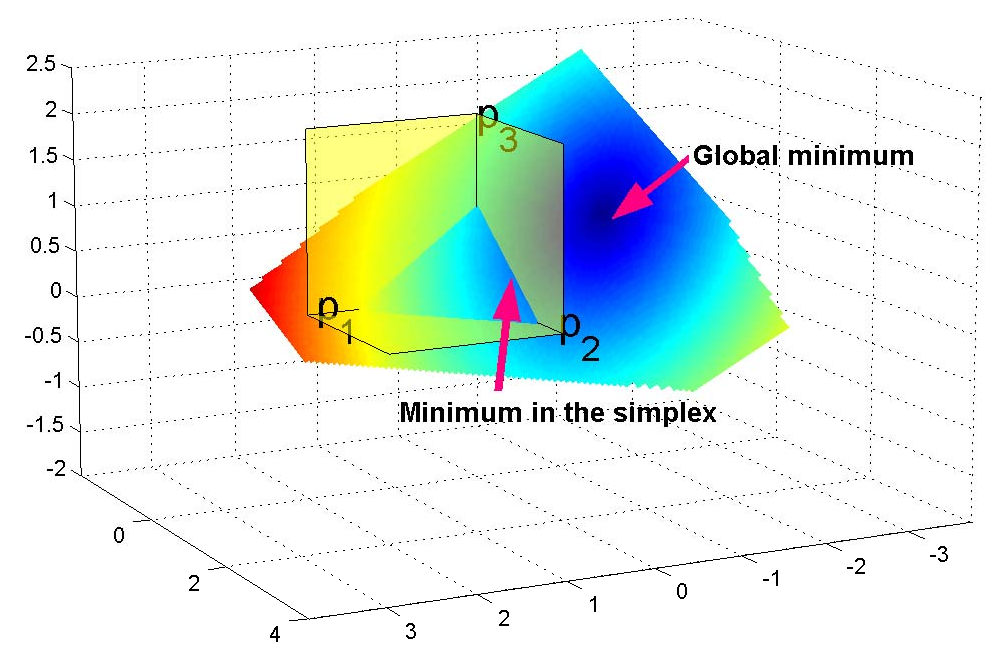
\includegraphics[width=\fwB]{img/CvxMinSimplex}
%  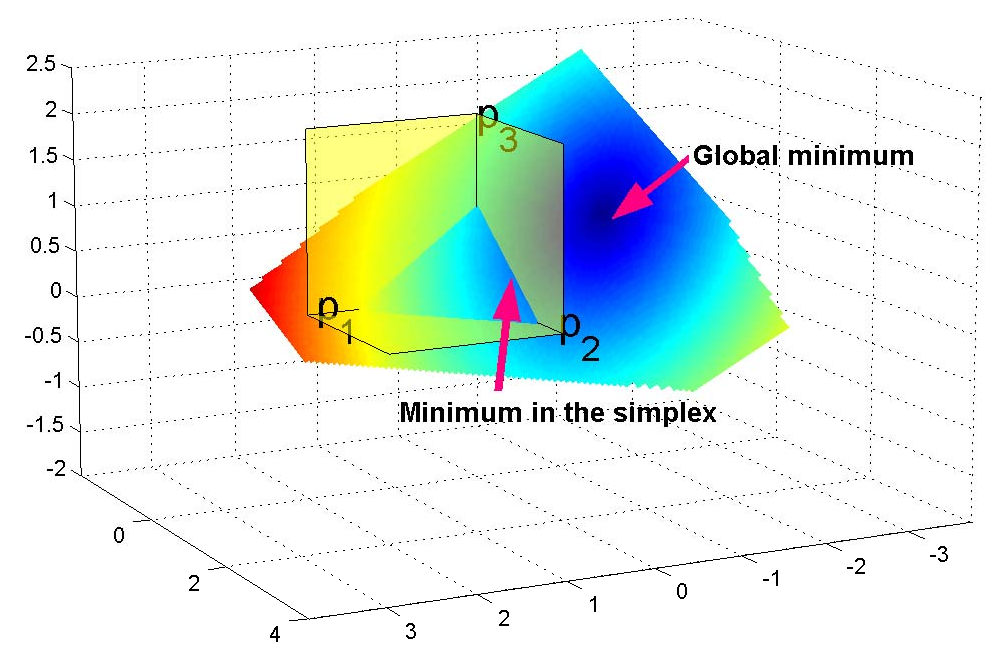
\includegraphics[width=\fwB]{img/CvxMinSimplex}
  \caption{A geometric interpretation on Lemma~\ref{t:outofmin}.}\label{f:outofmin}
\end{figure}
    In this 3D example, $p_1$, $p_2$ and $p_3$ are the axes. The parameter equation for the sliding surface is $p_1+p_2+p_3=1$. The simplex $\mathbb{S}_P$ is the triangle inside the $(p_1,p_2)$, $(p_2,p_3)$, and $(p_1,p_3)$ plans. The color of the sliding surface indicates the value of a cost function: The value of the cost function increases as the color changes from blue to red. The triangle is a convex set. If there exists a global minimum point with the gradient equals to $\mathbf{0}$ (stationary point), Lemma~\ref{t:outofmin} says that the global minimum point is out of the triangle, which is the same as Fig.~\ref{f:outofmin}. It is easy to see that the minimal value within the triangle, $\mathbb{S}_P$, must take place on the boundary of the triangle.


    Actually, for our sensor selection problem, the stationary point ($\nabla_{\mathbf{p}}\Psi = 0$) is infinite far away, where $\mathbf{p}\rightarrow \infty$ and $M^{-1} \rightarrow 0$. In other words, the estimation error is totally rejected if we take infinite number of samples.
    It is easy to see that the minimum value on the triangle must take place on the boundary of the triangle. While the 3D example is straightforward, we need to prove that such relations are still true for arbitrary high order.
\end{remark}

Next, we claim that $\mathbb{S}_M$ is convex for arbitrary high order. Since it is convex, the Carath\'{e}odory's theorem is valid on the set. Due to limited space, the proofs of several following theorems are ignored.

\begin{lem}\label{t:cvx}
$\mathbb{S}_M$ is a convex set.
\end{lem}
\begin{proof}
We want to prove the follows: if
$$M(\mathbf{p}_1)\in\mathbb{S}_{M}, M(\mathbf{p}_{2})\in\mathbb{S}_{M},$$
 and $$ \bar{M}=\alpha M(\mathbf{p}_{1})+(1-\alpha)M(\mathbf{p}_{2})$$ then $\bar{M}\in\mathbb{S}_{M}$,
where $\alpha\in\mathbb{R},\alpha\in[0,1]$.

Define $$\mathbf{p}_T := \alpha\mathbf{p}_1+(1-\alpha)\mathbf{p}_2.$$
If $$M(\mathbf{p}_{1})\in\mathbb{S}_{M} \mathrm{\ and\ } M(\mathbf{p}_{2})\in\mathbb{S}_{M},$$
then we have
\begin{eqnarray*}
\bar{M} & = & \sum_{i=1}^{n}\mathbf{p}_{T(i)}\mathbf{a}_{i}\mathbf{a}_{i}^{T}, \\
\end{eqnarray*}
Easy to see
$$\sum_{i=1}^{n}\mathbf{p}_{T(i)}=\alpha\sum_{i=1}^{n}\mathbf{p}_{1(i)}+
(1-\alpha)\sum_{i=1}^{n}\mathbf{p}_{2(i)},$$
$$\sum_{i=1}^{n}\mathbf{p}_{T(i)}=\alpha+(1-\alpha)=1.$$
So, $\bar{M}\in \mathbb{S}_M$.
\end{proof}


Since $\mathbb{S}_M$ is convex, the Carath\'{e}odory's theorem is valid on the set.
\begin{thm}[Carath\'{e}odory's theorem, based on~\cite{SilveyOptimalDesign1980}, p.72]\label{t:cara}
Let $\mathbb{S}$ be a subset of $\mathbb{R}^{n}$. Every element $\mathbf{x}$ in $\mathbb{S}$ can be expressed as a convex combination of no more than $n+1$ elements
of $\mathbb{S}$. If $\mathbf{x}$ is on the boundary of $\mathbb{S}$, $n+1$ can be replaced by $n$.
\end{thm}
\begin{remark}
An illustration on the  Carath\'{e}odory's theorem in 2D domain is shown in Fig.~\ref{f:cara}. In the figure, points A to G are 2D points within the same convex hull. According to the Carath\'{e}odory's theorem, no more than 3 supporting points are required to express any point in the convex hull. It is intuitive to see that point F can be expressed as a convex combination of points A, B, and E, since F is inside the triangle ABE. This convex combination may not be unique. The point F can also be expressed by points A, C, and E. Note the words of ``no more than.'' The point F is inside the convex hull and not on the boundary, but it can also be expressed as the convex combination of 2 points: i.e., points A and G.

Point B is on the boundary. According to the Carath\'{e}odory's theorem, it can be expressed by no more than two points. It is easy to see that point B can be expressed by points A and C.

\begin{figure}
  % Requires \usepackage{graphicx}
    \centering
  \includegraphics[width=\fwC]{img/CaraIllu}\\
  \caption{An illustration of Carath\'{e}odory's theorem in 2D domain. }\label{f:cara}
\end{figure}
\end{remark}


% Due to limited space, we do not include the proof for theorems that are not our contributions.

We still need several theorems in order to prove that our COSS algorithm selects the minimum number of sensors that allowed by the Carath\'{e}odory's theorem.

\begin{thm}[Based on \cite{PazmanOED86}, p.81]\label{t:DoptCvx}
The D-optimality criterion is convex if $M$ is non-negative definite and strictly convex if $M$ is positive definite.
\end{thm}

Now, we extend the above theorem.

\begin{cor}\label{t:DoptStrictCvx}
If $\Psi(M)$ is the D-optimality criterion, where $M$ is as Definition~\ref{d:SampRateOpt}, then $\Psi(M)$ is strictly convex.
\end{cor}
\begin{proof}
Check the proof of our Theorem~\ref{t:outofmin}. Since  $M$ is positive definite, according to Theorem~\ref{t:DoptCvx}, the $\Psi(M)$ is strictly convex.
\end{proof}
\begin{remark}
As we are going to see in the proof of Theorem~\ref{t:minsen}, the convexity of $\Psi(M)$ is important. A strict convex function has at most one unique minimum solution.
\end{remark}


\begin{thm}[Based on \cite{BertsekasNP99}, p.571] \label{t:cvxUnique}
If $\mathbb{S}\subset \mathbb{R}^n$ is a convex set and $g:\mathbb{S}\mapsto \mathbb{R}$ is a convex function, then a local minimum of $g$ is also a global minimum. If in addition $g$ is strictly convex, then there exists at most one global minimum of $g$.
\end{thm}


The multiplicative updating law in COSS can find the minimal solution, due to the following theorem.

\begin{thm}[Based on \cite{PazmanOED86}, p.140 and \cite{UcinskiOptDPS05}, p.65] \label{t:nodescreasing}
The multiplicative updating law (
               $p_{i}[j+1]=p_{i}[j]\frac{\phi_{i}(\mathbf{p}[j])}{m}$ )
in Algorithm~\ref{a:COSS} is nondecreasing. That is
$$ \lim_{j\rightarrow \infty} \det(M) = sup_{\mathbf{p}\in\mathbb{S}_P} \det(M),$$
where $j$ is the iteration number.
\end{thm}


Finally, we are ready to prove that our COSS algorithm selects the minimum number sensors that are allowed by the Carath\'{e}odory's theorem.


\begin{thm}\label{t:minsen} % m(m+1)/2 sensor enough
When $Rank(A)=m$, the COSS algorithm (Algorithm~\ref{a:COSS}) selects no more than $m(m+1)/2$ sensors, where $m$ is the number of parameters for estimation. That is, no more than $m(m+1)/2$ entries of $\mathbf{\hat{p}}$ are larger than 0, as the iteration number comes to infinity.
\end{thm}
\begin{proof}
This theorem is an extension of Lemma~\ref{t:outofmin}, Lemma~\ref{t:cvx}, Theorem~\ref{t:cara}, Corollary~\ref{t:DoptStrictCvx}, Theorem~\ref{t:cvxUnique}, and Theorem~\ref{t:nodescreasing}: Theorem~\ref{t:nodescreasing} says that the multiplicative updating law finds the minimal point after enough iterations.
    Lemma~\ref{t:outofmin} says that there is no stationary point, where the gradient equals to 0, inside the simplex $\mathbb{S}_P$. So, Algorithm~\ref{a:COSS} must find a minimal point on the boundary of $\mathbb{S}_p$. The supporting points for $M$ are $M_i$, where
    $$M_i = \mathbf{a}_i \mathbf{a}_i^T, \; \mathbf{a}_i\in \mathbb{R}^m.$$
     Each supporting point is a vertex of the simplex $\mathbb{S}_p$,
    since when
    $$p_i=1, p_j=0 (i\neq j),$$
     we have $M=M_i$; or, the convex hull of those supporting points is $\mathbb{S}_M$.

    Note that $M_i$ are symmetric matrices with $m(m+1)/2$ unique entries. Based on Lemma~\ref{t:cvx}, $\mathbb{S}_M$ is a convex set and Theorem~\ref{t:cara} is applicable. According to  Theorem~\ref{t:cara}, there exits one solution to represent the optimal $M$ by a convex combination of no more than $m(m+1)/2$ supporting points.

Corollary~\ref{t:DoptStrictCvx} says that the D-optimization function is strictly convex. According to Theorem~\ref{t:cvxUnique}, the one solution predicted by the Carath\'{e}odory's theorem is the unique solution.

    In summary, Algorithm~\ref{a:COSS} finds the one and only one solution. Since the solution is on the boundary of the convex set $\mathbb{S}_P$, no more than $m(m+1)/2$ sampling rate $p_i$ is not zero.
\end{proof}

\begin{remark}
In practice, infinite number of iterations are not possible. Thus,  the practical solutions are always very close to the boundary but not perfectly on the boundary.
    According to Theorem~\ref{t:minsen}, if the solution is perfectly on the boundary, no more than 3 sensors are required for a 2D tracking system, where $m=2$. If the solution is close to the boundary but still within the simplex, no more than 4 sensors are selected for the same scenario. Remind that Theorem~\ref{t:cara} predicts that one more supporting point is required if the element, i.e., the desired $M$, is inside the simplex.

Normally, in our tracking experiments, we observed that 3 sensors have high sampling rates (more than 0.2, or 20\% of the total sampling rate), 1 sensor's sampling rate is in the middle, and the rest sampling rates are much smaller (less than 0.01).
  If 4 sensors are selected, we can tune our system to select no more than 3 sensors by increasing $h_S$ or decreasing $\eta$. The tuning drives the solution closer to the boundary of the simplex, thus less sensors are selected. The tuning is not difficult in practice.

    Remind that paper~\cite{isler06tase} is in consistent with our analysis (see Section.~\ref{s:intro}).

%It is interesting to see that, through experiments, paper~\cite{isler06tase} observers that ``the estimates obtained by four best sensors are as good as the estimates obtained from all sensors'' for tracking by camera-like sensors. It seems that this observation is in consistent with our theoretical analysis. Note that paper~\cite{isler06tase} takes a geometric approach but our algorithm is an algebraic approach.

A further study on Theorem~\ref{t:minsen} indicates that the key feature of the COSS algorithm is not the D-optimality criterion, nor the multiplicative algorithm.
As we see than in the proof of Theorem~\ref{t:minsen}, the details of the multiplicative method is not used. The reason why the COSS can select sensors is due to that fact that $\Psi(M)$ is a convex function on a convex set.
\end{remark}

The following theorem formally present our observation.

\begin{thm}\label{t:ioss}
For the problem in Definition~\ref{d:SampRateOpt}, if $\Psi(M)$ is convex, $Rank(A)=m$, and there exists an algorithm to find $\hat{\mathbf{p}}$, such that
\begin{equation}\label{e:phat}
\hat{\mathbf{p}} =\mathrm{argmin}_\mathbf{p} \Psi(M(\mathbf{p}; \hat{\mathbf{q}}_A[k])),     \end{equation}
then no more than $m(m+1)/2$ entries of $\hat{\mathbf{p}}$ are positive. If (\ref{e:phat}) is not minimized, then no more than $m(m+1)/2+1$ entries are positive.
\end{thm}
\begin{proof}
Based on Theorem~\ref{t:minsen}, the proof is trivial: Replace the ``multiplicative algorithm'' by the optimization algorithm which finds $\hat{\mathbf{p}}$, then this theorem is proved.
\end{proof}
\begin{remark}
This theorem reveals the existing of a class of implicit optimal sensor selection (IOSS) methods. Under the guidance of Theorem~\ref{t:ioss} more IOSS algorithms can be systematically designed. COSS is just a simple example of the many IOSS methods. It is our future work to design and compare more IOSS methods.

The theorem also gives us some guidance on parameter tuning of generic IOSS methods. Other IOSS methods can be tuned similar to that of the COSS. Please refer to the remarks of Theorem~\ref{t:minsen}.
% If there are more sensors selected, then we can increase the iteration numbers of the optimization, or increase threshold $h_S$.
\end{remark}

%\begin{mdef}[implicit optimal sensor selection]
%
%\end{mdef}

Remind that D-optimality criterion has similar properties to the A- and E-optimality criteria.
%If we use the A-optimality criteria to replace the D-optimality criteria in Eq.~\ref{e:dopt}, and replace the multiplicative method in Algorithm~\ref{a:COSS}, we can easily prove that the new algorithm selects no more than $m(m+1)/2$ sensors also, just follow the structure of Theorem~\ref{t:minsen}. The solution of the new algorithm should also approximates the CRLB.
    In this chapter, we focus on D-optimality criterion. In addition to the advantages of the D-optimality that we list after Definition~\ref{d:SampRateOpt}, the solution the the D-optimization, i.e., the multiplicative method, is simple and fast. It has potentials to be implemented on low-cost sensor nodes, where computation resources are very limited.

As an extension of Theorem~\ref{t:minsen}, we give a theorem on the sensor deployment density requirements and achievable energy save factor.
\begin{thm} % requirement on sensor density
If each point sensor detects targets in its vicinity with a radius of $r$, sensor deployment density is $\rho$, and the energy cost of turning on all the sensors is $e_A$, then the minimal sensor density required by the COSS algorithm
% implicit optimal sensor selection algorithm (such as the COSS algorithm)
is $\rho_L$, and its associated energy requirement is $e_S$.
\begin{eqnarray*}
\rho_L &=& \frac{m(m+1)}{\pi r^2}, \\
e_S &=& \frac{m(m+1)}{\pi r^2 \rho} e_A,
\end{eqnarray*}
where $m$ is the number of parameters under observation.
\end{thm}
\begin{proof}
When a target appears, all the sensors within its vicinity will detect it. The detection range is $r$. Based on Theorem~\ref{t:minsen}, the COSS algorithm selects no more than $m(m+1)$ sensors. Thus, within the disc with a radius of $r$, we need to deploy at least $m(m+1)$ sensors. The area covered by the disc is $\pi r^2$.
Easy to see that the minimal sensor density is $\rho_L$ with $\rho_L = \frac{m(m+1)}{\pi r^2}$.

Assuming there are $n$ sensors deployed in an area with the square $s$. Thus, the number of sensors being selected by the COSS algorithm is $\rho_L s$. Assuming the energy cost is uniformly spread among all the sensors, we have
$$e_S=(\rho_L\cdot s \cdot e_A)/n.$$
Thus $ e_S = ( m(m+1)\cdot e_A)/(\pi r^2 \rho).$
\end{proof}
\begin{remark}
This theorem gives a necessary condition for the COSS algorithm, or other IOSS methods, to work properly. This theorem provides guidance on sensor deployment. That is, the sensor density must be no less than $\rho_L$.
  What is $r$ in practice? $r$ is the detection range of a sensor and should be found based on the data sheet of the sensor.
    Remind the polynomial model in Definition~\ref{d:poly} has a constant named $y_L$. From the sensor characteristics plot, such as Fig.~\ref{f:SensorFit}, it is easy to find the distance that associated with $y_L$. This distance is the maximum allowed $r$.

\end{remark}

\section{Experiment Results}\label{s:experiment}
\subsection{Simulations}\label{s:sim}
Simulation results are shown in Fig.~\ref{f:SSpos35No3} to Fig.~\ref{f:SSposOut2}. In those simulations, 15 light sensors are spread 20.32 cm apart from each other. The sampling period, $t_S$, is 1 sec, and the total sample number is 100. The signal noise ratio (SNR) is    8 dbm. The a priori position in the figure is $\mathbf{q}_A$. The a priori confidence ellipsoid is plot based on $M_A$, the FIM that associated to $\mathbf{q}_A$. The real target is believed within the ellipsoid. The a posterior position is $\mathbf{q}_B$, which is computed after the sensor selection. It is clear that the a posterior estimation is more precise in this case. The location error of the a priori estimation is 5.5883 cm, while the error of the a posterior is 3.7749 cm. From Fig.~\ref{f:SSpos35psiNo3} we see that the algorithm converges fast. In this example, it only take 4 iterations for the sampling rates to converge close enough to the optimal value.
% It took about 8 ms to execute the sensor selection algorithm once for a network with 60 sensors. The algorithm is implemented in Matlab and the execution time is measured by the profile tool from Matlab. This speed is fast enough for many real-time target tracking applications.


\begin{figure}
  \centering
  \includegraphics[width=\fwB]{img/SS15SNR8Pos33p}
  \caption{A simulation based on the COSS algorithm.}\label{f:SSpos35No3}
\end{figure}

\begin{figure}
  \centering
  \includegraphics[width=\fwB]{img/SS15SNR8Pos35Psi}
  \caption{Convergence speed of the COSS algorithm.}\label{f:SSpos35psiNo3}
\end{figure}


Note that the COSS algorithm does not requires the sensors to be placed uniformly. 60 sensors are randomly placed for the example in Fig.~\ref{f:SSRandPos}. In this example, the positing error of the a priori estimate is 1.7038 cm and that of the a posteriori estimate is 1.6193 cm. The determinate of the FIMs that associated with the a priori and a posteriori estimates are 12.9581 and 10.9482, respectively.

The simulations indicate that the selected sensors are not necessarily the closest sensors to the target. In Figs.~\ref{f:SS60pos33},~\ref{f:SSRandPos}, and~\ref{f:dense}, the closest one sensor is actually not selected.
    Figure~\ref{f:lt} is the light field for the example in Fig.~\ref{f:SS60pos33}. We see that selected sensors have relatively high, but not the highest, light values.

Figure~\ref{f:SSposOut} and Fig.~\ref{f:SSposOut2} are some extreme cases to show the performance of the COSS algorithm. In the figures, the target is not inside the WSN. We see that when the target is out of the coverage of the WSN, but not too far away, the position estimate is still precise. When the target is too far away, both the a priori estimate measured by the LS method and the a posteriori estimate based on the sensor selection optimization can not locate the target properly.


\begin{figure}
  \centering
  \includegraphics[width=\fwB]{img/SS60pos33Bp}
  \caption{Sensor selection for a network of 60 sensors by COSS.}\label{f:SS60pos33}
\end{figure}

\begin{figure}
  \centering
  \includegraphics[width=\fwB]{img/SS60LightField}
  \caption{Light field.}\label{f:lt}
\end{figure}

\begin{figure}
  \centering
  \includegraphics[width=\fwC]{img/Dense60Rand1}
  \caption{An example of applying the COSS algorithm to randomly placed sensors.}\label{f:SSRandPos}
\end{figure}


\begin{figure}
  \centering
  \includegraphics[width=\fwB]{img/Dense60}
  \caption{Applying the COSS algorithm to densely deployed sensors.}\label{f:dense}
\end{figure}

\begin{figure}
  \centering
  \includegraphics[width=\fwB]{img/SSposOut}
  \caption{Target is out of the boundary of the WSN.}\label{f:SSposOut}
\end{figure}



\begin{figure}
  \centering
  \includegraphics[width=\fwB]{img/SSposOut2}
  \caption{Target is far out of the boundary of the WSN.}\label{f:SSposOut2}
\end{figure}


\subsection{Hardware Experiments}\label{s:hardware}
Since we introduced several approximations in the our algorithm, it is important to verify the validity of those approximations by our physical testbed. A picture of the testbed in shown in Fig.~\ref{f:SSPlatformPic}. In the testbed, 15 Tmote sky sensor nodes are placed under a halogen lamp. The sink Tmote sky node (not in the picture) is connected to a PC. A GUI is running on the PC.


\begin{figure}
  \centering
  \includegraphics[width=\fwA]{img/SSPlatformPic}
  \caption{A picture of our sensor selection testbed.}\label{f:SSPlatformPic}
\end{figure}

 Figures~\ref{f:ScreenShots2},~\ref{f:ScreenShots3}, ~\ref{f:ScreenShots4},~\ref{f:Screen1} and~\ref{f:Screen2} are captured frames from our movie~\cite{zhencossUrl}
 that demonstrates the testbed. Notation on Figures~\ref{f:ScreenShots2},~\ref{f:ScreenShots3}, and ~\ref{f:ScreenShots4} are manually added.
 Figure~\ref{f:ScreenShots2} shows the GUI running on the sink. Figure~\ref{f:ScreenShots3} shows the initial stage of the tracking. The track is clearly shown in Fig.~\ref{f:ScreenShots4}.
    The important frames of the movie are shown in Figs.~\ref{f:Screen1},~\ref{f:Screen2}.
        The picture at the left bottom is from a movie taken by a camcorder. The selected sensors are the green dots on the screen, the unselected sensors are the red dots. In the movie, we see that no matter the lamp is smoothly moving or suddenly shifting, the system can always track the lamp.

 Figures~\ref{f:Screen1} and \ref{f:Screen2} are frames from our movie~\cite{zhencossUrl} that demonstrates the testbed. The picture at the left bottom is from a video taken by a camcorder. The selected sensors are the green dots on the screen, the not-selected sensors are the red dots. No matter the lamp is smoothly moving or suddenly shifting, the system can always track the lamp.


\begin{figure}
  \centering
  \includegraphics[width=\fwB]{img/CommentSSscreen2}
  \caption{A screen shoot of our sensor selection testbed: The GUI.}\label{f:ScreenShots2}
\end{figure}

\begin{figure}
  \centering
  \includegraphics[width=\fwB]{img/CommentSSscreen3}
  \caption{A screen shoot of our sensor selection testbed: Tracking the lamp.}\label{f:ScreenShots3}
\end{figure}

\begin{figure}
  \centering
  \includegraphics[width=\fwB]{img/CommentSSscreen4}
  \caption{A screen shoot of our sensor selection testbed: The track.}\label{f:ScreenShots4}
\end{figure}


\begin{figure}
  %\centering
  \begin{center}
    \mbox{
      \subfigure[Frame 1]{\includegraphics[width=\fwC]{img/CompressedSenSelScreenShot0001}} \quad
      \subfigure[Frame 2]{\includegraphics[width=\fwC]{img/CompressedSenSelScreenShot0002}}
      }
    \mbox{
      \subfigure[Frame 3]{\includegraphics[width=\fwC]{img/CompressedSenSelScreenShot0003}} \quad
      \subfigure[Frame 4]{\includegraphics[width=\fwC]{img/CompressedSenSelScreenShot0004}}
      }
    \mbox{
      \subfigure[Frame 5]{\includegraphics[width=\fwC]{img/CompressedSenSelScreenShot0005}} \quad
      \subfigure[Frame 6]{\includegraphics[width=\fwC]{img/CompressedSenSelScreenShot0006}}
      }
    \caption{Screen shots for tracking mobile target using the sensor selection algorithm.}
    \label{f:Screen1}
  \end{center}
\end{figure}

\begin{figure}
    \begin{center}
    \mbox{
      \subfigure[Frame 7]{\includegraphics[width=\fwC]{img/CompressedSenSelScreenShot0007}} \quad
      }
    \caption{Frame 7 for tracking mobile target using the sensor selection algorithm.}
    \label{f:Screen2}
  \end{center}
\end{figure}


Comparing to the simulation, the hardware implementation is more challenging due to the following reasons:
\begin{itemize}
  \item Imperfect communications introduce packet drops.
%  \item Nonlinear light sensors. As we described before, the real sensors are nonlinear, which may introduce some errors to the system.
  \item Disturbances from the ambient light.
  \item The light bulb is not a perfect point light source. In fact, the size of the light bulb is about 3 cm, which is comparable to the tracking error of our testbed.
  \item The light reflector behind the light bulb is not perfect and the reflection is not very smooth. That is, the distribution on the light field is not perfect.
  \item The sensor noise is not an ideal Gaussian noise.
\end{itemize}


According to our experiment results, those approximations are valid under realistic application conditions. The algorithm is robust enough for us to demonstrate our system under different ambient light conditions. The system is also robust to other WiFi (IEEE 802.15.x) devices in our lab. No performance degradation is observed after introducing those WiFi devices in the vicinity of the testbed.
%    Fig.~\ref{f:ScreenShots2} is a marked frame that captured from our movie~\footnote{This movie and other experiment results are available at \url{http://cc.usu.edu/~zhensong/CDC07}.} that demonstrates the testbed.





Despite of those difficulties, we still achieve our goals: The COSS algorithm selects 3 sensors and, statistically, the a posteriori estimates are more precise than the a priori estimates. We measure the positioning errors on 21 points on the testbed.
    The indices of those 21 points are shown in Fig.~\ref{f:indices}.
\begin{figure}[!h]
  \centering
  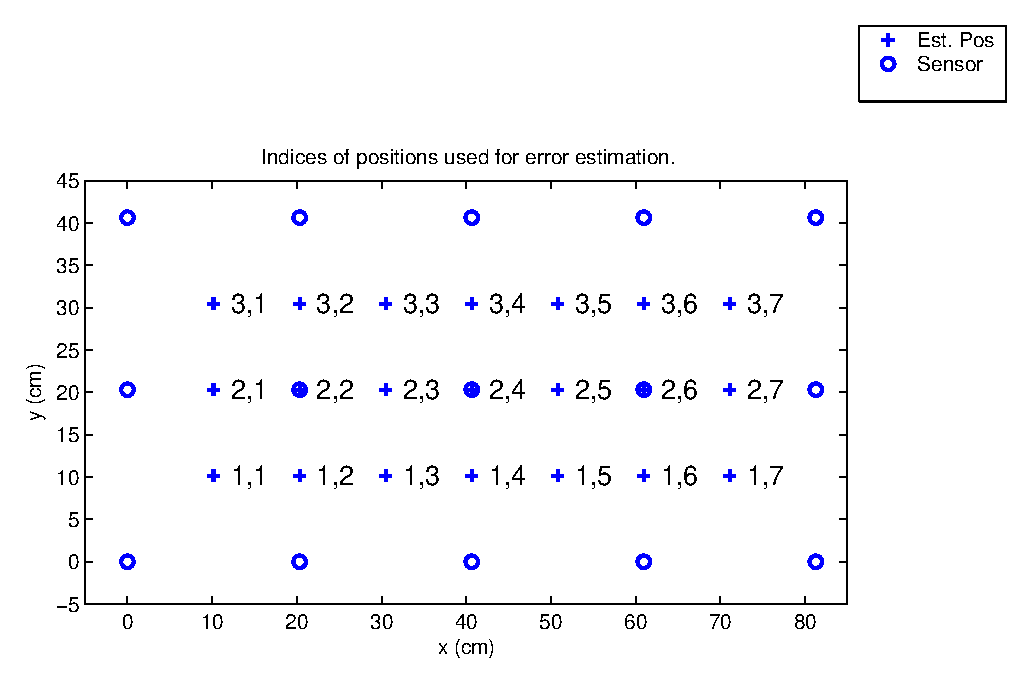
\includegraphics[width=\fwB]{img/IndexPosErrorEst}\\
  \caption{Indices of positions used for error estimation.}\label{f:indices}
\end{figure}
    After placing the lamp on one of those positions, we manually measure the position and take it as the real position. The a priori and a posteriori positions are logged in a data file.
        Figure~\ref{f:SSHardwareErrorSurf} is plotted based on those experiment data. The mean tracking error for the a priori estimate is 3.1387 cm, and the mean error for the a posteriori estimate is 3.0269 cm.
 Not surprisingly, the advantages of the a posteriori estimates over the a priori estimates in the hardware experiments are not as significant as that in the simulations. This is due to the listed hardware imperfectness.
    The upper two plots in Fig.~\ref{f:SSHardwareErrorSurf} are drawn in scale. We see that the positing error, or the height in the $z$-axis, is very small. In order to show see the positing error clearly, the two lower plots in Fig.~\ref{f:SSHardwareErrorSurf} have enlarged $z$-axis.


On Fig.~\ref{f:SSHardwareRatioSurf} the ratio of the a posteriori estimation error over the a priori estimation error is plot as a surface. Thus, the COSS improves estimation precision at those places where that ratio is lower than 1. In the figure, we see that on most positions the error of the a posteriori estimate is smaller than that of the a priori estimate. Although the error of the a posteriori estimate is not always smaller than that of the a priori estimate, the a posteriori estimates are better for most of the area.


Figures~\ref{f:SSHardwareMovieFrame1to6}, ~\ref{f:SSHardwareMovieFrame7to12},~\ref{f:SSHardwareMovieFrame13to18}, and~\ref{f:SSHardwareMovieFrame19to21} are captured from a movie~\cite{zhencossUrl}
which is rendered based on the same experiment data that Fig.~\ref{f:SSHardwareErrorSurf} and Fig.~\ref{f:SSHardwareRatioSurf} use. The plots in Figs.~\ref{f:SSHardwareMovieFrame1to6}, ~\ref{f:SSHardwareMovieFrame7to12},~\ref{f:SSHardwareMovieFrame13to18}
,~\ref{f:SSHardwareMovieFrame19to21} have information that have not been presented in Fig.~\ref{f:SSHardwareErrorSurf} or Fig.~\ref{f:SSHardwareRatioSurf}. The manually measured positions of the lamp, the selected sensors, the a priori and a posteriori position estimates.


\begin{figure}
  \centering
  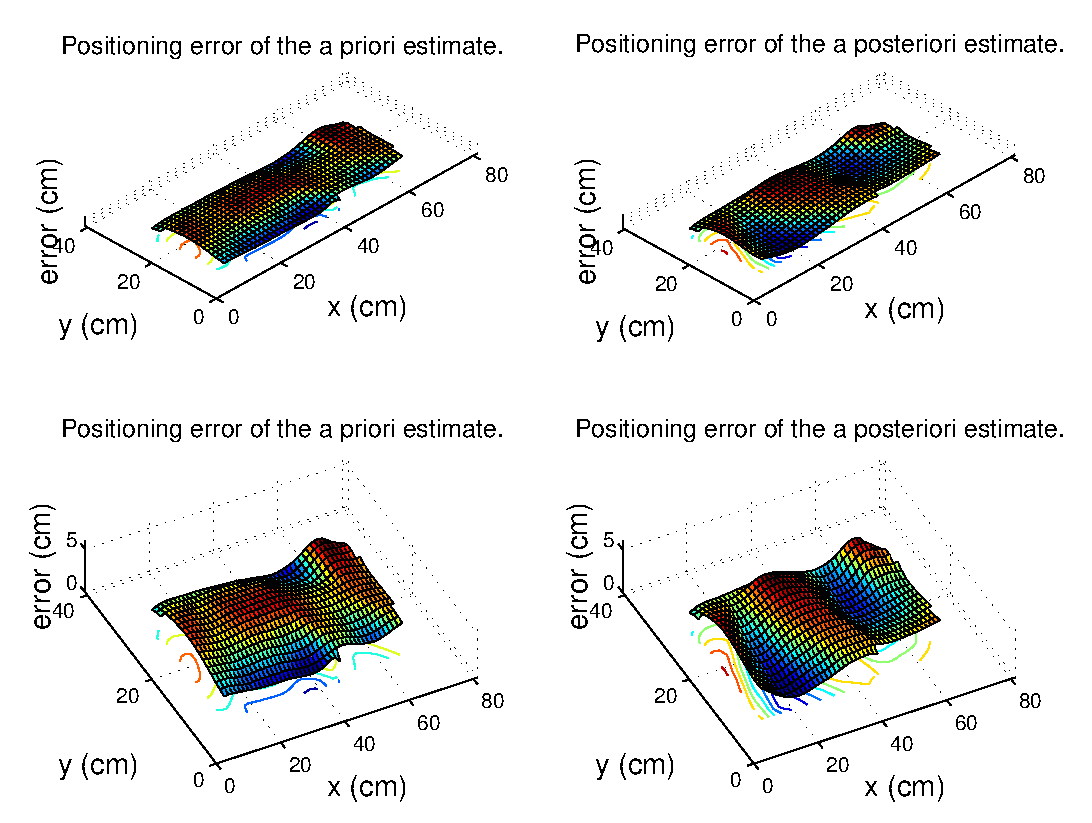
\includegraphics[width=\textwidth]{img/SSHardwareErrorSurf4plotsP}
\caption{Estimation errors of our sensor selection testbed.}\label{f:SSHardwareErrorSurf}
\end{figure}


\begin{figure}
  \centering
  \includegraphics[width=13cm]{img/SSHardwareRatioSurfP}
\caption{A ``before-and-after'' comparison of our sensor selection testbed: ratio of the a posteriori estimation error (after sensor selection) over the a priori (before sensor selection) estimation error.}\label{f:SSHardwareRatioSurf}
\end{figure}





\begin{figure}[!h]
  \centering
    \mbox{
      \subfigure[Position (1,1)]{\includegraphics[width=\fwC]{img/SSHardwareMovieFrame1}} \subfigure[Position (1,2)]{\includegraphics[width=\fwC]{img/SSHardwareMovieFrame2}}
      }
    \mbox{
      \subfigure[Position (1,3)]{\includegraphics[width=\fwC]{img/SSHardwareMovieFrame3}} \subfigure[Position (1,4)]{\includegraphics[width=\fwC]{img/SSHardwareMovieFrame4}}
      }
    \mbox{
      \subfigure[Position (1,5)]{\includegraphics[width=\fwC]{img/SSHardwareMovieFrame5}} \subfigure[Position (1,6)]{\includegraphics[width=\fwC]{img/SSHardwareMovieFrame6}}
      }
    \caption{Hardware testing results for sensor selection: positions (1,1) to (1,6).}
    \label{f:SSHardwareMovieFrame1to6}
\end{figure}
%\clearpage


\begin{figure}[!h]
  \centering
    \mbox{
      \subfigure[Position (1,7)]{\includegraphics[width=\fwC]{img/SSHardwareMovieFrame7}} \quad
      \subfigure[Position (2,1)]{\includegraphics[width=\fwC]{img/SSHardwareMovieFrame8}}
      }
    \mbox{
      \subfigure[Position (2,2)]{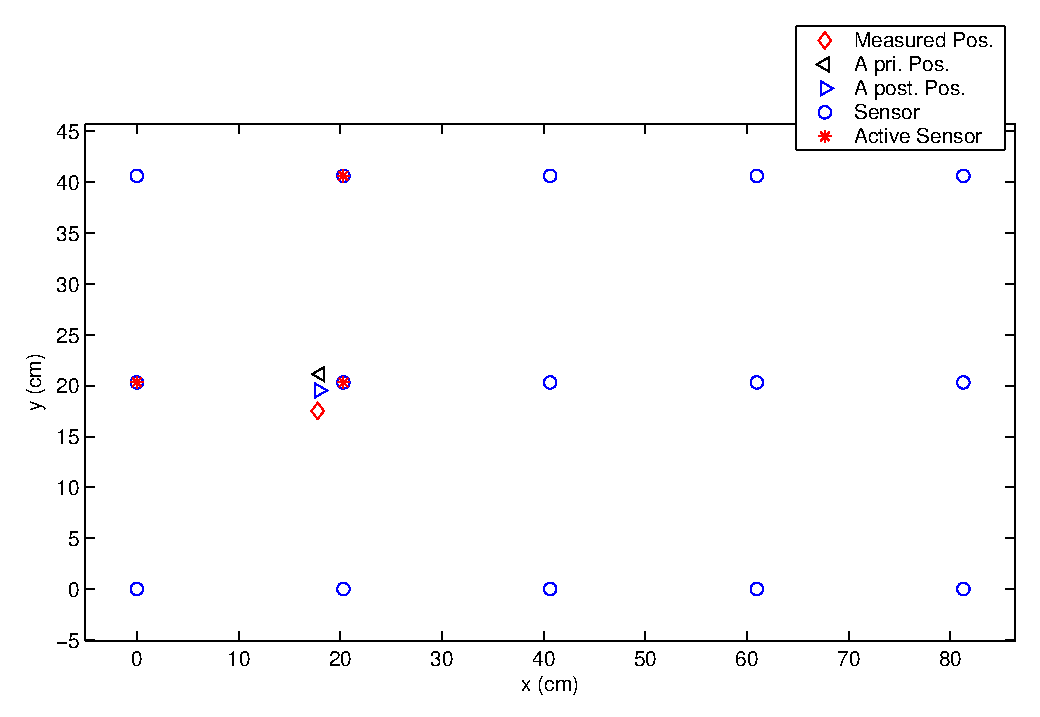
\includegraphics[width=\fwC]{img/SSHardwareMovieFrame9}} \quad
      \subfigure[Position (2,3)]{\includegraphics[width=\fwC]{img/SSHardwareMovieFrame10}}
      }
    \mbox{
      \subfigure[Position (2,4)]{\includegraphics[width=\fwC]{img/SSHardwareMovieFrame11}} \quad
      \subfigure[Position (2,5)]{\includegraphics[width=\fwC]{img/SSHardwareMovieFrame12}}
      }
    \caption{Hardware testing results for sensor selection: positions (1,7) to (2,5).}
    \label{f:SSHardwareMovieFrame7to12}
\end{figure}
%\clearpage


\begin{figure}[!h]
  \centering
    \mbox{
      \subfigure[Position (2,6)]{\includegraphics[width=\fwC]{img/SSHardwareMovieFrame13}} \quad
      \subfigure[Position (2,7)]{\includegraphics[width=\fwC]{img/SSHardwareMovieFrame14}}
      }
    \mbox{
      \subfigure[Position (3,1)]{\includegraphics[width=\fwC]{img/SSHardwareMovieFrame15}} \quad
      \subfigure[Position (3,2)]{\includegraphics[width=\fwC]{img/SSHardwareMovieFrame16}}
      }
    \mbox{
      \subfigure[Position (3,3)]{\includegraphics[width=\fwC]{img/SSHardwareMovieFrame17}} \quad
      \subfigure[Position (3,4)]{\includegraphics[width=\fwC]{img/SSHardwareMovieFrame18}}
      }
    \caption{Hardware testing results for sensor selection: positions (2,6) to (3,7).}
    \label{f:SSHardwareMovieFrame13to18}
\end{figure}


\begin{figure}[!h]
  \centering
    \mbox{
      \subfigure[Position (3,5)]{\includegraphics[width=\fwC]{img/SSHardwareMovieFrame19}} \quad
      \subfigure[Position (3,6)]{\includegraphics[width=\fwC]{img/SSHardwareMovieFrame20}}
      }
    \mbox{
      \subfigure[Position (3,7)]{\includegraphics[width=\fwC]{img/SSHardwareMovieFrame21}} }
    \caption{Hardware testing results for sensor selection: positions (3,5) to (3,7).}
    \label{f:SSHardwareMovieFrame19to21}
\end{figure}

\afterpage{\clearpage}


\section{Discussion}\label{s:diss}
\subsection{Remarks on the Speed and Memory Requirements}\label{s:remarks}
% add speed comparison
 The COSS algorithm is simple, fast, and memory efficient.

Comparing to other related methods, the COSS algorithm is simple and fast.
We use the Profile tool from Matlab and test the speed of our Matlab version COSS algorithm. On a 3Ghz Pentium 4 PC with 1Gb memory, it takes the COSS algorithm around 8 ms to optimize a network with 60 sensors. In our testbed, the COSS algorithm is implemented by the C\# language and execute in real-time. After the sensor nodes submit their data to the sink, no delay can be observed before the sink selects the sensors based on the COSS and broadcast the results to the sensor nodes.
% The implementation in C\# is likely to be even faster than that of the Matlab. However, due to the complexities of our software, we have not segmented the algorithm from other code and measured the real speed of the algorithm.

    It is reported in~\cite{SAM2006Amit} that the sensor selection based on B\&B integer programming method ``allows us to schedule up to 50-60 sensors typically in the order of seconds.'' In~\cite{isler06tase}, the sensor selection patterns are computed off-line and stored in a look-up table. That paper says that ``in an application where less than six sensors must be allocated per target, the $O(n^5)$ running time may be prohibitive for real-time implementation.''





% In addition, since only an array is being updated by the multiplicative law, the complexity of the COSS algorithm is $O(n)$. Comparing to a heuristic entropy based sensor selection method in~\cite{wang04entropybased}, the complexity of the algorithm is $O(k^2),$ there $k$ is the grid number in each dimension. $k$ could be very high under high-resolution cases. The COSS has a lower complexity.

The COSS algorithm requires memory to store $\nabla_{\mathbf{q}} \Psi$, $M$, and $\mathbf{a}_i$. Thus, it requires memory for $2mn+m^2$ float or double variables, where $m$ is the number of parameters and $n$ is the sensor number. This is a small number with respect to the grid-based methods. Since $m$ is small ($m=2$ or 3 for tracking problems) the required memory is not much. %, COSS requires 1Kb to 2Kb memory for a network with 60 sensors.
    Considering grid-based Bayesian or entropy approaches, those methods need memory to store $k^2$ or $k^3$ cells, where $k$ is the number of cells in each dimension.
    %    In~\cite{liu02collaborative}, it is claimed that (for the IDSQ sensor selection method) ``we need to compute mutual information from three-dimensional joint density ... This may be computationally intensive given the limited ability of sensor nodes.'' %Comparing those methods, the proposed COSS algorithm is more memory efficient, especially for high-resolution parameter estimation applications.


%Since the complexity and memory requirement of the COSS algorithm is linear to the number of sensors, this algorithm has good scalability: the execution time and memory requirement increase linearly with respect to the number of sensors.
\subsection{Comments on Non-Gaussian Noises}~\label{s:gauss}
The formation of FIM in (\ref{e:FIM}) is derived under the assumption that the sensor noise is Gaussian. The derivation of the FIM is presented in Appendix B. What if the noise is not Gaussian?
 In practice, non-Gaussian noise is not unusual.
    The question can be answered from theoretical analysis and hardware experiments.

From the theoretical aspect, the side effects of the non-Gaussian noise can be compensated by larger number of samples.
    There are connects between the Gaussian and non-Gaussian noises. It is claimed in~\cite{EmeryOED98} that ``since the covariance error matrix for independent Gaussian distributed errors is the same as the asymptotic covariance matrix of any distribution~\cite{Goodwin1977} it is usual to assume that the errors are Gaussian.''  Comparing Gaussian and Non-Gaussian is a rich topic. Further discussion is out of the scope of this dissertation.
        Based on the aforementioned result, if there are enough number of samples, the solution of minimizing the covariance matrix of independent Gaussian noises applies to non-Gaussian noises as well.
     %       On the other hand, it is not easy to find a threshold number such that the non-Gaussian noises can be considered as Gaussian once the sample number is larger than the threshold.
         In practice, we can increase the number of samples if the estimation precision is not satisfied.


Under this context, it is valuable to test the algorithm on a physical testbed with non-Gaussian sensor noise. In fact, our experimental data indicates that the sensor noise is not ideal Gaussian.
 Based on the hardware experiments, we observed that the COSS algorithm is not sensitive to the non-Gaussian noise.  However, under this condition, the a posteriori estimates are still more precise than that of the a priori estimates.

    Hereby we study the distribution of the sensor noise.
    Figure~\ref{f:hist3d} includes the plots of noise's histogram. During the experiments, Tmote Sky sensor nodes are placed under a halogen lamp at 11 positions whose ranges are uniformly distributed. 100 samples per distance are collected. One histogram can be drawn for each distance. For easy comparisons, the centers of those histograms are shifted to 0 and they are plotted in 3D figures.
      The 11 histograms are plots as 11 curves in Fig.~\ref{f:hist3d}(a) and Fig.~\ref{f:hist3d}(b). The histograms are also plotted by 3D surface in Fig.~\ref{f:hist3d}(c) and Fig.~\ref{f:hist3d}(d). The sensor data that collected at ranges closer than 30 cm have irregular histograms.
      % The histograms have several humps and the center of the histograms are not on humps. Thus,
      The sensor noises are not always Gaussian.
%     It is seen that the histograms from sensors whose distance is about 30 cm to 50 cm are Gaussian-like: Although they may have more than one humps per curve, the central humps are significantly higher than the side lobes.
%      However, the sensor data that collected at ranges closer than 30 cm have irregular histograms. The noises are not Gaussian-like. In summary, the noise is not
    Fig.~\ref{f:hist3dflor} is the same as Fig.~\ref{f:hist3d} except under different lamps. All the data in Fig.~\ref{f:hist3d} is collected under a halogen lamp, while Fig.~\ref{f:hist3dflor} is scenario under a florescent lamp. It is easy to see that the non-Gaussian noise exists under both of the situations.

In summary, although the COSS algorithm is derived based on Gaussian noise, the method is also applicable to non-Gaussian noises. Although some error may be introduced. The claim is supported by existing theory~\cite{EmeryOED98} and our extensive hardware experiments.

\begin{figure}
  \centering
  \subfigure[Front view.]{\includegraphics[width=0.4\textwidth]{img/Hist3DFront}}
  \subfigure[Top view.]{\includegraphics[width=0.4\textwidth]{img/Hist3DSideTop}}
  \subfigure[Side view.]{\includegraphics[width=0.4\textwidth]{img/HistSurf3DSide}}
  \subfigure[Top view.]{\includegraphics[width=0.4\textwidth]{img/HistSurf3DTop}}
  \caption{3D plots of the sensor noise histogram. (under a halogen lamp)}\label{f:hist3d}
\end{figure}


\begin{figure}
  \centering
  \includegraphics[width=0.7\textwidth]{img/FloreHisto}
  \caption{3D plots of the sensor noise histogram. (under a florescent lamp)}\label{f:hist3dflor}
\end{figure}

\subsection{Relationships with Geometric Approaches}\label{s:geo}
The sensor selection method in~\cite{isler06tase} is based on pure geometric approaches. Therefore we compare our algebraic approach with the geometric approaches.

Figure~\ref{f:alggeo} illustrates the rough ideas of the two methods. The geometric method is depicted in Fig.~\ref{f:alggeo}(a) and Fig.~\ref{f:alggeo}(b). The rest plots are associated with the algebraic method.
\begin{figure}
  \centering
  \includegraphics[width=\textwidth]{img/GeoVsAlg}\\
  \caption{Comparing the algebraic and geometric interpretations on estimation errors.}\label{f:alggeo}
\end{figure}
    A camera-like sensor studied in~\cite{isler06tase} can be characterized as a cone in Fig.~\ref{f:alggeo}(a). The angular estimation error on the target is the same as the angle of the cone. At least two sensors are required in order to estimate the position of the target, i.e., $(x,y)$. Figure~\ref{f:alggeo}(b) depicts the example when two sensors locate the position of a target.
        The estimation error is defined as the overlapping region~\footnote{It is called the minimum enclosing parallelogram (MEP) in~\cite{isler06tase}.} of the cones, since the estimate on the position of the target must fall inside both of the cones. As more sensors introduced, the overlapping region is a convex polygon~\cite{isler06tase}. It is proved in Lemma 4 of~\cite{isler06tase} that no more than 6 sensors are required in order to reduce the area of the overlapping region to be no more than twice of the minimum area.


Consider the algebraic approach using our formulation. Assuming the real position of the target is $(0.5,0.5)$.
 In Fig.~\ref{f:alggeo}(c) the only one sensor's measurement is $\theta_A=45^\circ$, which is corrupted by additive Gaussian noise $v$, and $v\sim \mathcal{N}(0,\sigma)$. The sensor's position is at $(0,0)$. The possible positions of the target, based on $\theta_A$ only, are indicated by the stars.



There are two angular sensors in Fig.~\ref{f:alggeo}(d). Their positions are $(0,0)$ and $(1,0)$, and their nominal angular measurements are $\theta_A=45^\circ$ and $\theta_B=135^\circ$, respectively. $\theta_A$ and $\theta_B$ are contaminated by independent Gaussian noise. After simple computations we have:
\begin{eqnarray*}
% \nonumber to remove numbering (before each equation)
  \hat{x} &=& \frac{-\tan(\theta_B)}{\tan(\theta_A)-\tan(\theta_B)}, \\
  \hat{y} &=& \frac{-\tan(\theta_A)\tan(\theta_B)}{\tan(\theta_A)-\tan(\theta_B)}.
\end{eqnarray*}
In other words, one position, $(\hat{x},\hat{y})$, can be estimated from one tuple of the angular measurements, $\{\theta_A, \theta_B\}$.
 Each star in Fig.~\ref{f:alggeo}(d) is associated with an estimated position, i.e., $(\hat{x}, \hat{y})$. It is seemed that the stars roughly fall inside an ellipse, which can be parameterized by a $2\times 2$ covariance matrix. Since the noise in Fig.~\ref{f:alggeo}(d) is Gaussian the envelop of those stars are more like an ellipse than a polygon.
  If more sensors are introduced, the position can be estimated by LS or WLS methods, and the size of the covariance is unchanged. Refer to (\ref{e:mb}) for details. For our algebraic approach, the estimation errors are always measured in ellipsoids whose dimensions are the same as that of the parameters under estimation.


 Easy to see that the ellipsoid area with starts in Fig.~\ref{f:alggeo}(d) is an approximation to the overlapping polygon region in Fig.~\ref{f:alggeo}(b). %In fact, the difference between the two does not necessarily make the optimizations based on ellipsoids less accurate than the polygon approach.
 Under certain conditions, the optimization on the ellipsoids is the same as the optimization on the polygons. Remind,~\cite{EmeryOED98} suggests that independent Gaussian distributions can be used to estimate the covariance matrix of any distribution.
%  It is claimed in~\cite{EmeryOED98}: ``Since the covariance error matrix for independent Gaussian distributed errors is the same as the asymptotic covariance matrix of any distribution~\cite{Goodwin1977} it is usual to assume that the errors are Gaussian.''
% % Thus, when there are enough number of samples, the problem of minimizing covariance matrices of any distribution can be converted into a problem of minimizing the covariance matrix of independent Gaussian noises.


 Take a look at Fig.~\ref{f:alggeo}(e) and Fig.~\ref{f:alggeo}(f), which are the cases when the noises are subjected to uniform distributions.
    Except that the noise is uniformly distributed, Fig.~\ref{f:alggeo}(e) is the same as Fig.~\ref{f:alggeo}(c). The stars in Fig.~\ref{f:alggeo}(f) are estimated target positions. The envelop of those stars is the same as the polygon in Fig.~\ref{f:alggeo} (b). Since the noises are uniform, the algebraic method in Fig.~\ref{f:alggeo}(f) is comparable to a Monte Carlo approach to compute the polygon in Fig.~\ref{f:alggeo}(b).
As aforementioned, under proper conditions, the optimization on the covariance matrix of the stars in Fig.~\ref{f:alggeo}(d) is the same as that in Fig.~\ref{f:alggeo}(f). The similarity between Fig.~\ref{f:alggeo}(d) and Fig.~\ref{f:alggeo}(b) is obvious. Thus, the difference between Fig.~\ref{f:alggeo}(b) and Fig.~\ref{f:alggeo}(d) may not as significant as they looked. % and they may be dual problems.

The interesting fact is that the observations from the two different approaches are in consistent with each other.
    It is observed in~\cite{isler06tase} that ``the estimates obtained by the four best
sensors are as good as the estimates obtained from all sensors.
Hence, the lifetime of the network can be significantly increased
by restricting the number of active sensors to a small number
without losing too much from the quality of the estimates.''
    Follow the algebraic approach, we conclude that no more than $m(m+1)/2+1$ sensors are good enough to provide the optimal estimate, for the worst cases. That is, when the sampling rate optimization is not optimized. (For the optimal solutions, $m(m+1)/2$ sensors are required. Check Section.~\ref{s:analysis} for the details.) When a target is in a 2D domain, $m=2$, and the $m(m+1)/2+1$ is exactly four!
Despite of the similarities, there are some difference between the two approaches:
\begin{itemize}
  \item The polygon representations of the geometric approach may be more precise than the ellipsoid of the algebraic approach, for example, when the sensor noise is uniformly distributed.
  \item It is easier to consider high-dimensional systems by the algebraic approach. For example, if there are 4 or more parameters need to be estimated, it is not easy to draw overlapping polygons and compute their areas. For the algebraic approach, the change is trivial. Only adjust the size of the matrices.
  \item Replacing different cost functions in the geometric method (currently there is only one cost function) is not as easy as that in the algebraic method. This is explained in the following paragraphs.
  % The algebraic approach has more options on the cost function for the optimization. The optimization criteria of algebraic approach is not necessarily the area of the overlapping polygons. The geometric interpretations on different optimality criteria of the algebraic approach is discussed in the following paragraph.
\end{itemize}

In the remark of Definition~\ref{d:SampRateOpt}, several optimality criteria are listed. They all have geometric interpretations. Hereby we explain them under the scenario in Fig.~\ref{f:alggeo}.
    The output of the D-optimality is proportional to volume of the covariance matrix, i.e., the area of the star clouds in Fig.~\ref{f:alggeo}(d) and Fig.~\ref{f:alggeo}(f). The geometric meaning of the D-optimality criterion is the same as the area of the overlapping region in~\cite{isler06tase}.
The D-optimality is the most widely used criterion and its advantages are described after the Definition~\ref{d:SampRateOpt}. However, it is not perfect. For example,  it is possible that the volume of a covariance matrix is small but the positioning error is significant. For example, when the confidence ellipsoid is very tall or wide. Under those cases, the A-optimality, which indicates the positioning error measured in Euclidean distances, or E-optimality, which is proportional to the maximum diameter of the confidence ellipsoid, are desirable options. Since E- and A-optimality criteria are not invariant to linear transforms, we may need to scale measurements into common units before applying the optimality criteria. For more discussions on other optimality criteria, such as the C-, T-, Tuning, and MV criteria, refer to~\cite{EmeryOED98,UcinskiCDC05}.


\subsection{Entropy-based Method}
The so called entropy-based methods in this dissertation can be interpreted intuitively: The sensor data which enhance the certainty on the estimate of the target's position is useful, and the sensors whose data is useful should be selected.
    The theory of Shannon entropy and Bayesian theory play central roles for some sensor selection methods~\cite{liu02collaborative,FZhaoShinInfoDrivenDynamicTracking,zhao03collaborative,wang04entropybased,ErtinMaxMutualInfoIpsn03}.
This approach is also referred as the information theoretic method~\cite{wang04entropybased}.
% To avoid ambiguity, we refer the approach as entropy-based method in Fig.~\ref{f:ssChart}. % This method is briefly compared with our proposed method is Section~\ref{s:intro}, hereby we compare them in more advanced topics.

Roughly speaking, the Shannon entropy is comparable to the covariance matrix of the COSS. The LS fitting in COSS method plays the same rule as that of the Bayesian theory in the entropy-based method.

The IDSQ algorithm~\cite{liu02collaborative} is an example of the entropy-based methods. In this method, the belief on the position of a target is updated according to sequential Bayesian filtering. Based on the measurement of information, i.e., entropy, the sensor within the vicinity of estimated target position and provides the ``most information'' is selected. A heuristic interpretation on the entropy is as the follows: The selected sensor have the largest number of bits to contribute to the estimation on the target's new position. Comparing to IDSQ, the COSS follows a different logic: The gradient in Fisher information is a metric of sensitivity. The valuable information contained in sensor data is measured by the sensitivity of the sensor readings with respect to the physical parameters under observation. If a sensor is ``sensitive'' to the parameter, its reading changes significantly due to the perturbations on the parameter. In plain words, the COSS method selects sensors that are most sensitive to the target's position (or other parameters). The Bayesian filtering in IDSQ is similar to the LS in COSS, in the sense they both update estimates based on sensor data. Of course, they are also significantly different since the target's dynamics can be considered under the framework of Bayesian filtering, but not under the LS.


Table~\ref{t:comp} compares the IDSQ and the proposed COSS algorithms. As we see, most entries of them are complementary. The followings are some remarks on the table.

The IDSQ is fully distributed, which is an advantage over the COSS method. Although the
COSS has potential to be implemented in a fully distributed fashion, most of the
computation of the COSS method is currently carried out by the sink, and the sensor nodes are responsible for a small part of the computation.
Note that, the distributed D-optimization and LS fitting have been developed~\cite{MurrayDecActiveSensing,XiaoBoydLallp2p_ls}.

The dynamics of the target are considered by the IDSQ method, due to the sequential Bayesian filter. Currently, the dynamics are not included in the COSS, and it is our future work is to incorporate distributed Kalman filter-like algorithms within the COSS, similar to~\cite{ChhetriSchedulingTrackingPhD2006,SabermobileDKF_cdc06}.
    Kalman filter can be consider a special Bayesian filter. A significant differences between the two is that the Kalman filter is not grid-based algorithms, but the Bayesian filter is. Since the COSS method is also not grid-based, it is compatible with the Kalman filter. The original Kalman filter is centralized and subjected to Gaussian noise. Currently, there are distributed Kalman filters~\cite{SabermobileDKF_cdc06} and the Gaussian noise is not mandatory.
    % Thus, the Kalman filter and the Bayesian approaches should have similar outputs when there is one unbiased estimate on the parameter.


One obvious difference is that the IDSQ is a grid-based algorithm while the COSS is not. The IDSQ method requires several 2D meshes to store the probability mass functions. The higher the resolution, the more the grids are required.
    On the contrary, the COSS only requires two arrays to store the sampling rates and sensitivities of each sensor. The length of the arrays is determined by the number of sensors. It may be faster and less demanding on the memory.

Both methods accept the non-Gaussian sensor noise, but due to different reasons. The IDSQ method is grid-based, thus nonparametric. Any probability distribution can be represented by the grids. The COSS is a parametric non-grid-based method and deduced based on Gaussian noise. However, as Section~\ref{s:gauss} presents, non-Gaussian noise may be acceptable, with some scarifies on the estimation precision.

The key feature of the COSS method is that it optimizes the estimate with a small number of sensors. That is, the estimation error is close to CRLB and the number of selected sensors is determined by the Carath\'{e}odory's theorem. For the IDSQ, the most ``informative'' one sensor is selected. If all the sensors are selected, the Bayesian method (in the IDSQ) provides the ``maximum a posteriori'' (MAP) estimate on the parameter. The MAP estimate is close to LS estimate under many conditions~\cite{EmeryOED98}. Intuitively, if only one sensor is selected, the estimate may not better than the MAP estimate.

Finally, both methods have been tested by hardware. The IDSQ testing scenario is outdoor vehicle tracking. The COSS has been test by the aforementioned testbed.

% Such a kind of feature is not discussed by IDSQ or similar entropy-based methods. For example, within the framework of IDSQ, it is not trivial to analyze the gain on estimation precision if top three most ``informative'' sensors are selected, instead of the best one sensor.


% The COSS estimates the position with LS. Comprehensive comparisons among Bayesian method, maximum likelihood, and least squares is presented in~\cite{EmeryOED98}. If all the sensors are selected, the Bayesian method provides the ``maximum a posteriori'' (MAP) estimate on the parameter. The MAP estimates may be biased; While the estimate by LS is always unbiased, if the unbiased estimator exists~\cite{EmeryOED98}. For additive Gaussian noise, the estimated parameter with the maximum likelihood (ML) is the same as the LS estimate. Thus, the estimated parameters of the COSS method are the ML estimate. In short, the estimated parameters of the IDSQ method approximate to MAP estimate. While the COSS method provides ML estimates.
% The method of IDSQ and COSS happens to represent two types of parameter estimation approaches: Bayesian and maximum likelihood methods, respectively. The target's position is estimated by sequential Bayesian filtering by the IDSQ method. If all the sensors are selected, the Bayesian method provides the ``maximum a posteriori'' (MAP) estimate on the parameter. While the


% Before the discussion, let us clarify a confusing term: entropy. Note that Appendix~\ref{s:fi} introduces the Fisher information entropy, which is a metric that indicates the ``order'' of a partial system. This is related to the classical thermodynamic entropy, which indicates the disorder of molecules. The Shannon entropy is an example of information entropy and was motivated to measure the amount of information that lost during transmission. Whether there are connections between the two entropies is out of the scope of this paper. Some authors believe there are connections between the two, while others do not. % Also notice the minute difference between the ``information'' of the information entropy (Shannon entropy) and the ``information'' of the Fisher information.


\begin{table}
\caption{Comparisons on IDSQ and COSS Methods.}\label{t:comp}
\begin{tabular}{| l ||c|c|}
  \hline
  % after \\: \hline or \cline{col1-col2} \cline{col3-col4} ...
  {\bf Properties} & {\bf IDSQ} & {\bf COSS }\\
  \hline\hline
  Target dynamics & yes & no \\
  Fully distributed & yes & no \\
  Grid-based method & yes & no \\
  Computation cost & high & low \\
  Memory requirements & high & low \\
  Accept non-Gaussian noises & yes & yes, but some precision is sacrificed \\
  Estimation precision in theory & unknown & close to CRLB \\
%  Unbiased estimate & not guaranteed & guarantee to find it, if it exists \\
  Number of selected sensors & one at a time & guided by the Carath\'{e}odory's theorem \\
%  Type of the estimate & MAP & ML\\
  Hardware experiment & yes & yes \\
  \hline
\end{tabular}
\end{table}

%  The role of the Shannon entropy in those papers is comparable to the role of Fisher information or FIM in our paper. As we see in the appendix~\ref{s:fi}, there is a Fisher information entropy. Is there any connection between the Shannon entropy and the Fisher information entropy? What is the relationships between the Shannon entropy-based and the FIM-based sensor selection methods? These natural questions can not be easily answered in one sentence. Roughly speaking, the Fisher information entropy is associated with thermothermodynamic entropy. The Shannon entropy-based sensor selection method is comparable to the lossless compression methods, such as the one used in Zip files. The FIM-based sensor selection method is comparable to the lossy compression method used by MPEG compressions.



%\begin{figure}
%  % Requires \usepackage{graphicx}
%  \centering
%  \includegraphics[width=\textwidth]{img/FiVsEntropy}\\
%  \caption{Comparing entropy and Fisher information.}\label{f:entropyFIM}
%\end{figure}

% \subsection{Maximum Likelihood vs. Max A Posteriori}

% \subsection{Grid or Non-Grid Method}


\subsection{Discussions on Correlations of Sensor Data}
One of the assumptions in this chapter is that the sensor noises are independent. Such an assumption is important for the analysis in Section~\ref{s:gauss} and Section~\ref{s:geo}. In the following paragraphs, we argue that such assumption is reasonable.

In the following paragraphs, we firstly present our experiment data and draw conclusion from the data that the sensor noises are independent. Then our simulations indicate that the dependency among noises can be canceled by properly designed hardware systems.
% Finally, we discuss whether the dependency, if it exists, should be considered by high-level optimization or be canceled in low level designs.

The dependency of the sensor noise can be measured by the correlations of the sensor data.
Remind that the correlation between random variables, $X$ and $Y$, is measured by the correlation coefficient $\rho_{X,Y}$.
    \begin{equation*}\label{e:rhoxy}
        \rho_{X,Y} =\frac{E\{(X-\mu_X)(Y-\mu_Y)\}}{\sigma_X \sigma_Y},
    \end{equation*}
    where $\mu_X$, $\mu_Y$ are the mathematical expectations of the random variables, and the $\sigma_X$ and $\sigma_Y$ are the standard deviations. Thus, if the sensor noises
%~\footnote{Strictly speaking, the statement is valid for unbiased sensor noises. The requirement on the unbiased sensor noise is not a strong assumption. If the sensor noise is not unbiased in practice, it can be calibrated, for example, by a lookup table.}
    are $v_X$ and $v_Y$, we have $v_X=X-\mu_X$ and $v_Y=X-\mu_X$.
% When sensors are close each other, $\mu_X$ and $\mu_Y$ are similar. However, $v_X$ may or may not have any relationship with $v_Y$. The COSS algorithm requires the noise to be independent, that is
    If and only if the sensor noises are independent, the following equation holds:
    \begin{equation*}\label{e:ind}
        E\{v_X v_Y\} = E\{v_X\}E\{v_Y\}.
    \end{equation*}
%    Thus, independent sensor noise implies $\rho_{X,Y} = 0$ when $X\neq Y$, and $\rho_{X,Y} = 1$ when $X=Y$.


%    {\it \textbf{for discussion only}
%    Paper~\cite{VuranSpatioTemporal04} claims that densely deployed sensors are subject to spatial correlations since ``multiple sensors record information about a single event in the sensor field. Due to high density in the network topology, spatially
%proximal sensor observations are highly correlated
%with the degree of correlation increasing
%with decreasing internode separation.'' We argue that the redundance among the sensor data does not necessarily introduce correlations. }

    One may think that the correlation between sensor data increases as the inter-sensor distance reduces. This intuition is wrong. When the sensors are close to each other, their measurements are close. However, those sensor data may or may not be correlated.
      Fig.~\ref{f:cor} is a visual interpretation on the claim. Suppose two sensors are so close to each other that their measurements, $X$ and $Y$, have the same expectation (mean), or $\mu_X \approx \mu_Y$. Figure~\ref{f:cor} shows that $X$ and $Y$ may or may not be correlated. In Fig.~\ref{f:cor}(a) there are three point clouds, representing three set of measurements. The centers of the clouds, i.e., the expectations, are $(0,0)$, $(1,1)$, $(2,2)$. For sensor selection purposes, one out of the two sensors should be selected, since their mean measurements are the same.
     In Fig.~\ref{f:cor}(b), $X_i$ and $Y_i$ are the $i$th measurement of $X$ and $Y$, respectively. The contour in Fig.~\ref{f:cor}(b) represents the values of the correlation coefficients between $X$ and $Y$.
     As Fig.~\ref{f:cor}(b) indicates, $X_2$ and $Y_2$ are not correlated. $X_1$ and $Y_1$ have positive correlations, and $X_3$, $Y_3$ have negative correlations. In summary, no conclusion on the correlation can be drawn from the fact that $\mu_X \approx \mu_Y$.

\begin{figure}
  % Requires \usepackage{graphicx}
  \centering
  \includegraphics[width=\fwA]{img/EgCorr}\\
  \caption{Illustration on correlations.}\label{f:cor}
\end{figure}


    So, when the sensor data is correlated? In the context of sensor networks, we argue that {\it common impact factors} introduce correlations between sensor data. The so called common impact factors are the phenomena that influence many sensor measurements at the same time. A contradictory term is {\it local impact factors} which only affect one sensor's reading. Examples of the common impact factors include ambient light, room temperature, lamp flashing pattern, which will be discussed soon. Local impact factors include sensor node ADC quantization errors, battery imperfectness, sensor noise, etc.
        Why the common impact factors introduce correlations?
            It is due to the fact that the common impact factor perturbs the readings from different sensors with certain predictable trends.
                For example, if $X$ is increased due to the brighter ambient light, $Y$ should also increase due to the same ambient light. This case is similar to the 1st measure (at the position (0,0)) in Fig.~\ref{f:cor}, where $Y$ tends to increase while $X$ increases. Then, as aforementioned, $X$ and $Y$ are correlated.
            Comparing to the local impact factors, such as the quantization errors, there is no predictable trends among different sensors.
    When a sensor takes one measurement on the light value, some error is introduced due to the quantization of the ADC chip on the particular sensor node. No other sensors are affected by the same ADC chip.
      Hereby, no common trend between sensor data exists.
        Thus, there is no correlations between the sensors. This case is similar to the 2nd measure in Fig.~\ref{f:cor}.


Let us exam the statements based on our experimental observations. In addition, we give an example on how to cancel sensor data correlations, if they exist, based on our experiments.
 Fig.~\ref{f:corcoef}(a) is same as Fig.~\ref{f:sensorIID}. From these figures, we conclude that under halogen lamps, the light sensor measurements are statistically uncorrelated, since the absolute values for the coefficients of cross-correlations are close to zero.
    If we had chosen a florescent lamp, the degree of correlation among sensors is higher.


    Fig.~\ref{f:corcoef}(b) is the correlation coefficients for the light sensors on Tmote Sky nodes under a florescent lamp. This figure is also plot based on our experiment data.
    Unlike the halogen lamps or incandescent lamps, which do not flash, the florescent lamp flashes at the same frequency as the power line. (60Hz in the US.) Comparing Fig.~\ref{f:corcoef}(a) and Fig.~\ref{f:corcoef}(b), it is easy to see that the correlation of the sensors under the florescent lamp is more obvious. The mean absolute value of the correlation coefficients and the cross correlation coefficients of data under the florescent lamp is larger than that under the halogen lamp.
    From this aspect, the halogen lamp is better than a florescent lamp for our application.


 % In other words, if two sensors are placed under a halogen lamp, the sensing noise of one sensor does not help to characterize the other sensor's noise. At the moment when the reading of the first sensor is higher than the true value, due the the noise, the reading of the first sensor does not help us to improve the estimate on the second sensor. The probability for the second sensor to have higher or lower reading is no changed in the case. Our interpretation to the case is that the non-zero correlation coefficients reveal the existence of {\it common impact factors}, while the zero correlation coefficients indicates that measurements are affected by {\it local impact factors}, instead of common impact factors. For example, the quantization errors introduced from the circuits of each sensor node are local impact factors, meaning that the
%measurement error on one sensor node does not affect the readings of other sensor nodes. However, if the lamp is flashing, the sensor readings are affected by the flashing pattern, which is the common impact factor: The sensor readings raise and fall with the same pattern as the lamp is turned on and off. Thus, there are correlations among the sensor readings. If this is the case, we argue that the correlations should be eliminated by proper hardware designs or low-level filtering. For the aforementioned case, either a non-flashing lamp should be used or a software band-stop filter should be installed on the sensor, in order to reject the flashing signal. After adopting those proper techniques, the input data to the sensor selection algorithm should be uncorrelated.


We also simulate flashing lamps based on the experiment data. In addition to show that the flashing lamp is a common impact factor, the simulation also indicates that there could be many types of correlation patterns.
  Fig.~\ref{f:corcoef}(c) and Fig.~\ref{f:corcoef}(d) are plotted based on the simulation results. The scenario in Fig.~\ref{f:corcoef}(c) is as the follows: The flashing frequency is as half of the sampling rate of those sensors. At the time instances when the lamp is off, the sensors measure the ambient light, which is a constant. While the lamp is on, the measurement is the addition of the ambient and the lamp's light.
  If $\mathbf{d}_E$ is the data collected in experiment, and $\mathbf{d}_A$ is the simulated flashing light, then $\mathbf{d}_A$ is defined as:
\begin{eqnarray*}
  \mathbf{d}_A[2k] &=& \mathbf{d}_E[k], \\
  \mathbf{d}_A[2k+1] &=& c_A, \label{e:ca}
\end{eqnarray*}
where $c_A$ is a constant to simulate the ambient light, and $k$ is the trail number.
From Fig.~\ref{f:corcoef}(c) we see that the correlation among the sensor data are significant: Most of the correlation coefficients are either close to 1 or -1.
    Fig.~\ref{f:corcoef}(d) is the simulation for time-varying ambient light: The intensity of the ambient light follows a sinusoid signal, thus time-varying. The illumination of the lamp is steady. The readings from the sensors are the summation of the ambient light and the lamp's light.
If $\mathbf{d}_B$ is the simulated varying light, the following holds:
    \begin{eqnarray*}
      \mathbf{d}_B[k] &=& \mathbf{d}_E[k]+\mathbf{s}_A[k], \label{e:sA}
    \end{eqnarray*}
    where $\mathbf{s}_A[k]$ is a sinusoid function with respect to $k$.
    From Fig.~\ref{f:corcoef}(d), we see that the correlations among sensor data are also very high. However, the correlation pattern between Fig.~\ref{f:corcoef}(c) and Fig.~\ref{f:corcoef}(d) are different.

%In the simulations, the data correlation is increased as we introduce common impact factor to the sensor system. This result matches our observation that the correlation for sensor data under a florescent lamp is higher than that under a halogen lamp.

\begin{figure}
  \centering
  \subfigure[Exp. data for a halogen lamp.]{\includegraphics[width=0.4\textwidth]{img/HalogenCorrCoef}}
  \subfigure[Exp. data for a florescent lamp.]{\includegraphics[width=0.4\textwidth]{img/FloreCorrCoef}}
  \subfigure[Simulated flashing light.]{\includegraphics[width=0.4\textwidth]{img/SimFlashLtCorrCoef}}
  \subfigure[Simulated varying light.]{\includegraphics[width=0.4\textwidth]{img/SimVaryLtCorrCoef}}
  \caption{Correlation coefficients of sensor data.}\label{f:corcoef}
\end{figure}

Comparing Figs.~\ref{f:corcoef}(b),(c), and (d), we see that the correlation patterns could be significantly different and irregular. Since the correlation pattern changes as the common impact factor changes.
It is not likely to present all the possible correlations by several groups.
% Due to the complexities, our opinion is that it is desirable to cancel the correlation instead of developing a sensor selection method that compatible with correlated sensor data.
The reasons are as the follows:
% In fact, we have constructed other correlation patterns by replacing the $c_A$ in Eq.~\ref{e:ca} or the $\mathbf{s}_A[k]$ in Eq.~\ref{e:sA} by other functions. It is not likely to present all the possible correlations by only four groups, as shown in~\cite{VuranSpatioTemporal04,berger01objective}. % ???


%So far, we explained why the sensor data could be uncorrelated even when the sensors are densely deployed. What if the experiment data indicates the sensor measurements are correlated? Our suggestion is to revise the system design, instead of introducing an algorithm to handle the correlations. The reasoning is as the follows:

\begin{itemize}
  \item It is unacceptable for an engineering project to have unknown common impact factor. In stead of studying the statistics characteristics of the impact factor, the engineer must find out the source of the impact. Otherwise, the project is unreliable, since its success depends on some uncontrolled factor, which may be changed at any time.
  %  In practice, it is unacceptable if an unknown phenomenon has impacts on all the sensors.
  \item   After finding the common impact factor, we can cancel the factor by either hardware improvement or low-level filtering.
  Take our sensor selection testbed as the example, the dependency of the sensor noise can be canceled if the florescent lamp is replaced by a halogen lamp, or a software band stop filter which rejects 60Hz signals.
  \item As aforementioned, due to the complexities of the correlation pattern, it may be  difficult to develop a generic sensor selection method for a large class of correlations. After understanding the physics of the common impact factor, it is easier to reject the correlation at the lower level. Still take the flashing florescent lamp as the example, it is much easier to replace a lamp, rather than design a D-optimization method which does not require the independent sensor noises.
\end{itemize}

In summary, it is a reasonable to assume that the sensor noises are independent. If the raw sensor data is correlated, it may be desirable to cancel the correlation at the lower level.

% \subsection{On Optimization Theory}

\subsection{Comments on Networking}
Traditional networked communication systems are designed based on stacks, or layers. The layered structure of our sensor selection testbed is not presented by the system architecture in Fig.~\ref{fig:sysmodel}. For comparison purposes, the layered model of our sensor selection testbed is plotted in Fig.~\ref{f:stack}.


%The implementation of our sensor selection testbed mainly follows this model, but different.
One of the key features of this model is that the physical model plays an important role, as if a layer in the communication stack. Another key feature is that the parameter of communication layers is tuned by the observer layer. Thus the observer not only transmits and receives information from the communication stack, but also controls the stack.


As it can be seen in Fig.~\ref{f:stack}, the model of the physical world is required for the design of the observer, which is essentially the application layer of other communication models. The feature of this model is that a parameter of the communication stack, the transmission rate, is tuned by the observer. Remind that if a sensor is not selected, its transmission rate is zero. If it is selected, the rate is a constant.
Since the observer is model based, the parameter is in fact determined by the measurements on the physical world.

\begin{figure}[htb]
  % Requires \usepackage{graphicx}
  \centering
  \includegraphics[width=\fwB]{img/ModelWSNStack}\\
  \caption{Communication stacks of the COSS method.}\label{f:stack}
\end{figure}

% The COSS algorithm can be considered as a simple example of a cross layer model-based sensor network protocol. The relationship between a network parameter and the estimation precision is formulated as an optimization problem and solved. The design cross the boundary between the traditional application layer and the lower communication layers.


\section{Chapter Summary}\label{s:conclusion}
In this chapter, we proposed a COSS algorithm to solve the sensor selection problem.
    The algorithm not only selects the minimal number of sensors that allowed by the Carath\'{e}odory's theorem, but also pushes the estimation errors closer to the theoretical lower limit, i.e., the Cram\'{e}r-Rao lower bound. %This algorithm is simple, fast, memory efficient and scalable.
After extensive simulation and hardware experiments, we conclude that the approximations are reasonable for engineering practices.
    Our theoretical analysis reveals the existing of a class of sensor selection methods that are similar to the COSS method. They are named implicit optimal sensor selection method in this chapter.

In future, we will develop fully distributed COSS and implement it on low-cost sensor nodes for real-time target tracking.

%\appendix[Acronyms and Notations]\label{s:app}



%\section{Appendix: Acronyms and Notations}\label{s:app}
%%Since there are many acronyms and notations in this paper, we list them in below:
%
%\begin{itemize}
%\item LS: least square.
%\item WLS: weighted least square.
%% \item OED: optimal experiment design.
%\item FIM: Fisher information matrix.
%\item CRLB: Cram\'{e}r-Rao lower bound.
%\item WSN: wireless sensor network.
%\item vectors and matrices: vectors are typed in bold math font, such as vector $\mathbf{v}$. Matrices are indicated by capital math font, e.g., $M$. Note that random variable is denoted by bold capital font, e.g., $\mathbf{X}$. Thus, $\mathbf{p} \neq p \neq P \neq \mathbf{p}$, since $\mathbf{p}$ is a vector, $p$ is a scalar, and $P$ is a matrix. By default, all vectors are column vectors. For example, $\mathbf{p}=\left(
%                        \begin{array}{c}
%                          p_1 \\
%                          p_2 \\
%                          \vdots \\
%                          p_n \\
%                        \end{array}
%                      \right) = \left(
%                        \begin{array}{c}
%                          \mathbf{p}_{(1)} \\
%                          \mathbf{p}_{(2)} \\
%                          \vdots \\
%                          \mathbf{p}_{(n)} \\
%                        \end{array}
%                      \right).$
% Note that $\mathbf{p}_{(1)}$ is the first entry of the vector $\mathbf{p}$, and $\mathbf{p}_{(1)}$ is a scalar. $\mathbf{p}_1$ is a vector. By default, $M$ and $M_1$ are two difference matrices, and $M\neq M_1$.
%\item subscripts: the subscripts in brackets indicate scalar entries of a matrix or vector. The subscripts without brackets are instances of variables. Capital subscripts are parts of the variable's name. So, $t$ and $t_A$ are different scalars. Lower case subscripts, e.g., $i,j,k$, are used as indices for positive integers. For example, $\mathbf{p}_{(i)}$ is the $i$th entry of the vector $\mathbf{p}$, and $\mathbf{p}_{(i)}$ is a scalar.
%  Similarly, $M_{(i,j)}$ is the $i$th row and $j$th column scalar entry of matrix $M$. $M_{(i,:)}$ is the $i$th row vector of matrix $M$, and $M_{(:,i)}$ is the $i$th column vector of matrix $M$.
%    $\mathbf{p}_i$ is the $i$th $\mathbf{p}$ vector, where $i=1,2,3,\cdots$. Note that $p_i$ is the $i$th $p$, and $p_i$ is a scalar. Thus, $\mathbf{p}_i\neq p_i$.  However, $\mathbf{p}_{(i)}=p_i$ by default, and both of them are scalars. % Finally, this is a complex example: $M_{Ai(2,:)}^T$.
%\item $n$ : the total number of sensors. Note that $n\neq \mathbf{n}$.
%\item $n_i$, or $\mathbf{n}_{(i)}$: the number of samples that sensor $i$ collects in each $t_S$, the sampling period. Note that $\mathbf{n}=[n_1, n_2,\cdots]^T\neq n$. %when $i\neq0$, $n_i$ is the number of samples that sensor $i$ collects in $T_{t}$. At the initial stage, each sensor collect the same number of samples and send the average of the samples to sink. The initial number of samples is $n_0$. $n_0=c_t/N$.
%\item $P_r$: probability function.
%\item $m$: the number of parameter for identification.
%\item $t_S$: the total sampling time. In $t_S$, sensor $i$ collects
%$n_i$ samples.
%\item $n_{S}$: the max total number of samples of the whole WSN in $t_S$ time slot.
%\item $c_{1}$, $c_2$, etc: the coefficients in sensor model.
%\item $\sigma_{i}$, $\bar{\sigma}_{i}$, $\tilde{\sigma}_i$: $\sigma_{i}$ is the standard deviation of the noise of the $i$th sensor. $\bar{\sigma}_{i}$ is the standard deviation for the $i$th averaged sensor measurement. $\tilde{\sigma}_i$ is similar to $\bar{\sigma}_{i}$ but averaged over nominal sampling rates.
%%\item $f(k)$: the value of function $f$ at the time instance $k$.
%\item $f[k]$: the value of function $f$ for the $k$-th iteration.
%\item $y_i$ or $\mathbf{y}_{(i)}$: the nominal value of sensor $i$. It is computed by the model of events.
%\item $v_{i}$: the noise of sensor $i$.
%\item $s_i$ or $\mathbf{s}_{(i)}$: real value of the reading of sensor $i$. $s_{i}[k]:=y_{i}[k]+v_{i}[k]$.
%\item $\bar{s}_{i}$: averaged sensor $i$'s reading.
%\item $\mathcal{N}(\mu,\sigma)$: Gaussian (normal) distribution with the
%expectation of $\mu$ and variance of $\sigma$.
%\item $\mathbf{p}$: normalized sampling rate of sensor $i$. %As a variation,
%$\hat{\mathbf{p}}[k]$ is the optimized normalized sampling rate for the $k$-th iteration.
%\item $\mathbf{r}_{i}$: position of sensor $i$. $\mathbf{r}_{i}$ is assumed
%precisely known. In addition $\mathbf{r}_{i}\neq\mathbf{r}_{j}$,
%for any $i\neq j$. By default, $\mathbf{r}_{i}$ is a 2D vector like
%$\left(\begin{array}{c}
%x_{i}\\
%y_{i}\end{array}\right)$. % with $\mathbf{r}_{i(x)}=x_i$ and $\mathbf{r}_{i(y)}=y_i$.
%\item $\mathbf{q}$, $\mathbf{q}^\ast$: $\mathbf{q}$ is the position of the target. Specifically, $\mathbf{q}^\ast$ is the true position of the target.
%\item $\mathbf{1}$: an all-one vector, i.e., $[1, 1, \cdots, 1]^T$.
%\item $\nabla$: gradient. For example, $\nabla_{\mathbf{q}}$ is the gradient
%with respect to $\mathbf{q}$.
%\item $\mathbf{a}\geq b$: each entry of vector $\mathbf{a}$ is no less than the scalar $b$. $a_{i}\geq b$. E.g., $\mathbf{p}\geq 0$.
%\item $A\succeq B$: matrix $A-B$ is positive semi-definite.
%\end{itemize}




